% -*- TeX -*- -*- UK -*- -*- BMR -*-
% ----------------------------------------------------------------
% Beamer presentation ************************************************
% **** -----------------------------------------------------------
\documentclass[final]{beamer}%[handout][hyperref={backref=slide}]

\usepackage{array}
\usepackage{cancel}
%\input{sl_slide_preamble.tex}
\input{sl_slide_preamble_nonotes.tex}
%\usecolortheme[named=darkblue]{structure}
\usecolortheme[rgb={0.6372549 0.27843137 0.27058824}]{structure}
\setbeamercolor{alerted text}{fg=red!80!black}
\input{sl_slide_graphics_preamble.tex}
\input{sl_definitions.tex}
\input{sl_slide_symbols.tex}
%
\graphicspath{{"Figures/"}}
%================================================================================
\DeclareMathOperator{\SNR}{SNR}
\DeclareMathOperator{\snr}{SNR}
\newcommand{\snrb}{\overline{\snr}}
\newcommand{\syn}{\vec{w}}
\newcommand{\synid}{\syn_\text{ideal}}
%matrices
%prob vector
\newcommand{\pr}{\mathbf{p}}
%equilibrium distribution
\newcommand{\eq}{\boldsymbol{\pi}}
%first passage times
\newcommand{\fpt}{\mathbf{T}}
%off-diag first passage times
\newcommand{\fptb}{\overline{\fpt}}
%other symbols
\newcommand{\w}{\mathbf{w}}
\newcommand{\W}{\mathbf{W}}
\newcommand{\frg}{\W^\mathrm{F}}
\newcommand{\M}{\mathbf{M}}
\newcommand{\F}{\boldsymbol{\Phi}}
\newcommand{\wv}{\vec{w}}
%super/subscripts
\newcommand{\pot}{^{\text{pot}}}
\newcommand{\dep}{^{\text{dep}}}
\newcommand{\potdep}{^{\text{pot/dep}}}
%quantities
\newcommand{\initial}{\mathcal{I}}
\newcommand{\area}{\mathcal{A}}
\newcommand{\CS}{\mathcal{S}}
%================================================================================
%---------Title-----------------------------------------------------------

\title[Complex synapses]{Learning and memory with complex synaptic plasticity}
%
%\subtitle{\small{based on work with Surya Ganguli}}
%
\author{Subhaneil Lahiri%\inst{1}
}
%
\institute[Stanford]{%
%\inst{1}
Stanford University, Applied Physics
}
%
%\slideCaption{}

%---------Beginning--------------------------------------------------------

\begin{document}

%-------------Title--------------------------------------------------------

\begin{frame}
%
 \titlepage
%
\end{frame}
%================================================================================

%-------------Slide--------------------------------------------------------

\begin{frame}{What is a synapse?}
%
 \begin{center}
 \parbox[c]{0.45\linewidth}{
  %
%  \visible<3->{
  \begin{center}
    Experimentalists
  \end{center}
%  }
  %
 }
 \parbox[c]{0.45\linewidth}{
  %
%  \visible<2->{
  \begin{center}
    Theorists
  \end{center}
%  }
  %
 }

 \parbox[c]{0.45\linewidth}{
  %
%  \visible<3->{
  \begin{center}
    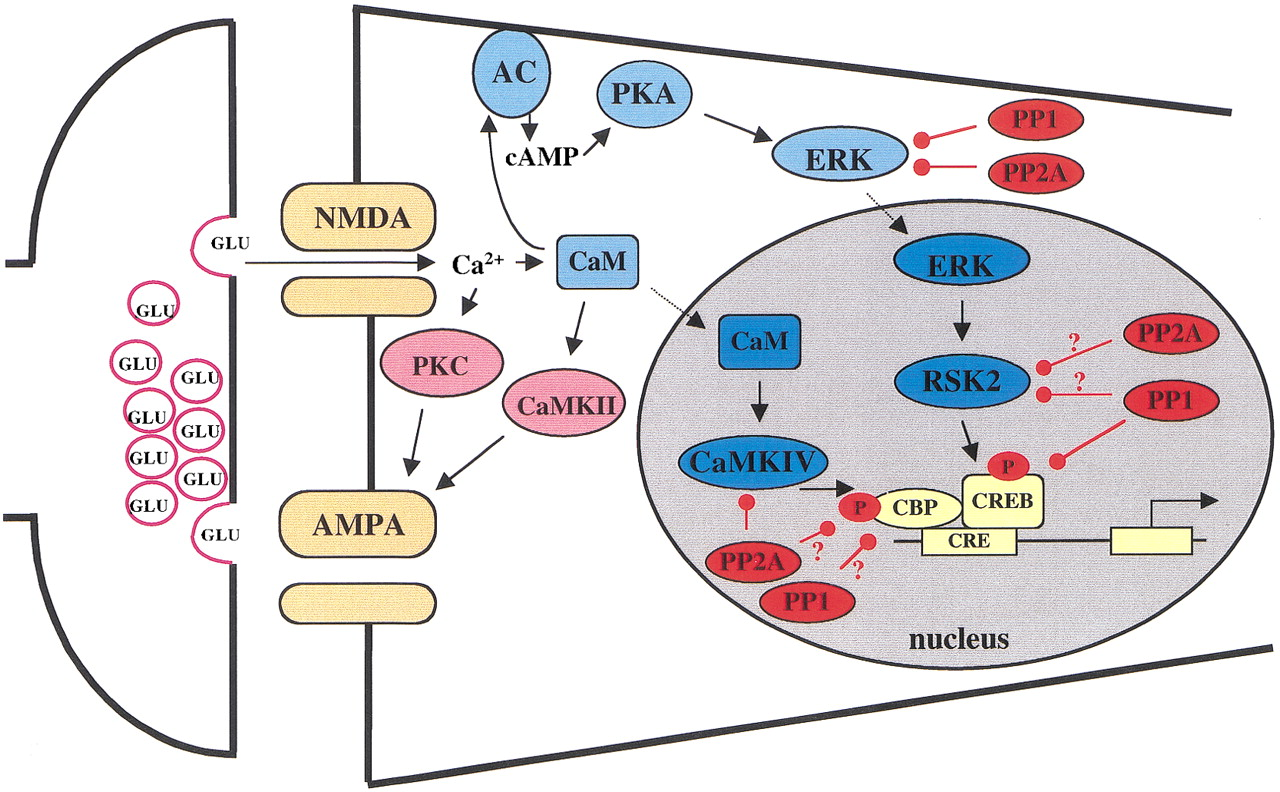
\includegraphics[width=0.95\linewidth]{plasticity-network.jpg}
  \end{center}
  %
  \citerr{Klann2002metaplasticity}
%  }
 }
 \parbox[c]{0.45\linewidth}{
  %
%  \visible<2->{
  \begin{center}
    \Huge $W_{ij}$
  \end{center}
%  }
  %
 }
 \end{center}
%
\end{frame}

%-------------Slide--------------------------------------------------------

\begin{frame}{Storage capacity of synaptic memory}
%
  Hopfield, perceptron have capacity $\propto N$, (\# synapses).

\vp\parbox[t]{0.59\linewidth}{%
  Assumes unbounded analogue synapses
  %Requires synapses' dynamic range also $\propto N$.

 \vp With discrete, finite synapses:\\
 $\implies$ memory capacity  $\sim\CO(\log N)$.
 \\ \citerr{amit1992constraints,amit1994learning}
 %
 }
 %
 \parbox[t]{0.4\linewidth}{
   %\begin{flushright}
    \hfill\aligntop{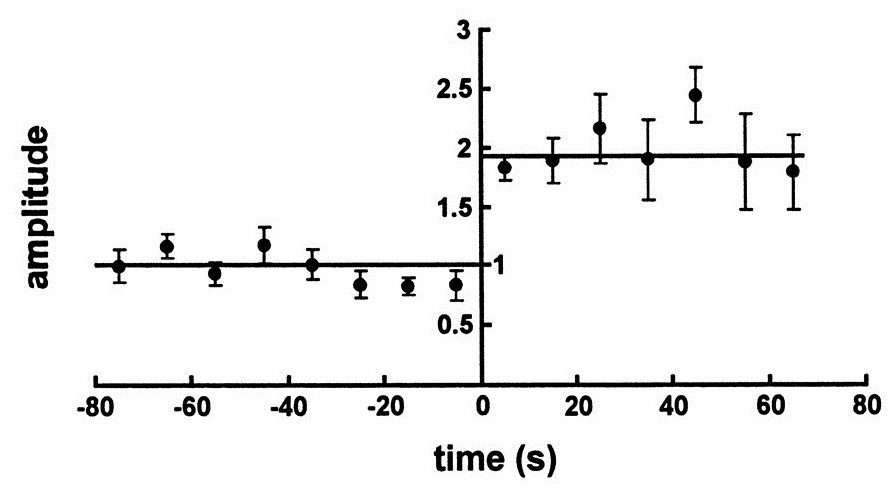
\includegraphics[width=0.9\linewidth]{Petersen1998.jpg}}
   %\end{flushright}
 }
 \\
    \citerr{Petersen1998allornone,OConnor2005switch}

% \vp When we store new memories rapidly,

 \vp New memories overwrite old
 \impl stability-plasticity dilemma.
 %
 \note[item]{or sparse $\sim \log N / N$}
%
\end{frame}

%-------------Slide--------------------------------------------------------

\begin{frame}{Synapses are complex}
%
 \parbox[t]{0.45\linewidth}{%
 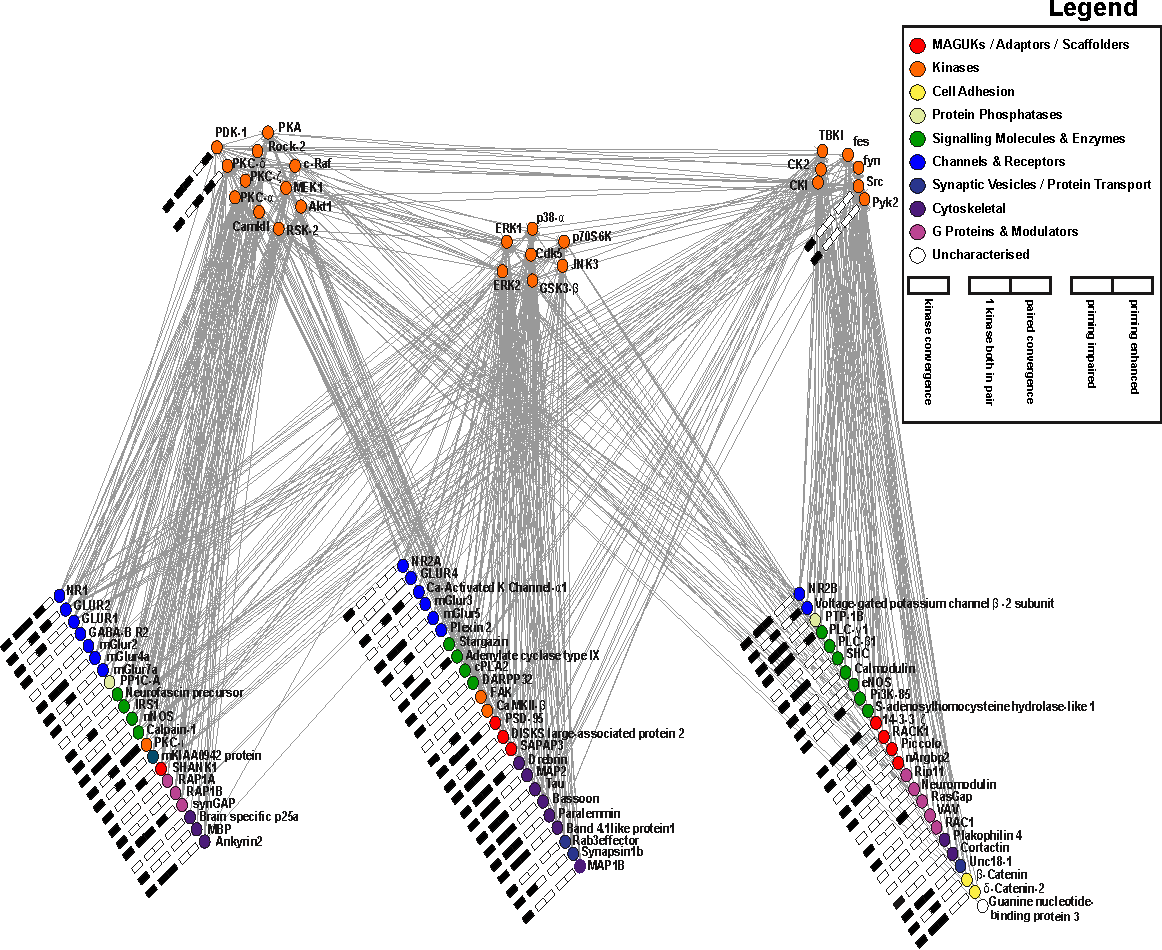
\includegraphics[height=0.8\linewidth]{2000102CobaFig4.pdf}

 \citerr{Coba2009phosphorylation}
 }
 \hspace{0.05\linewidth}
 \parbox[t]{0.45\linewidth}{%
 \hfill
 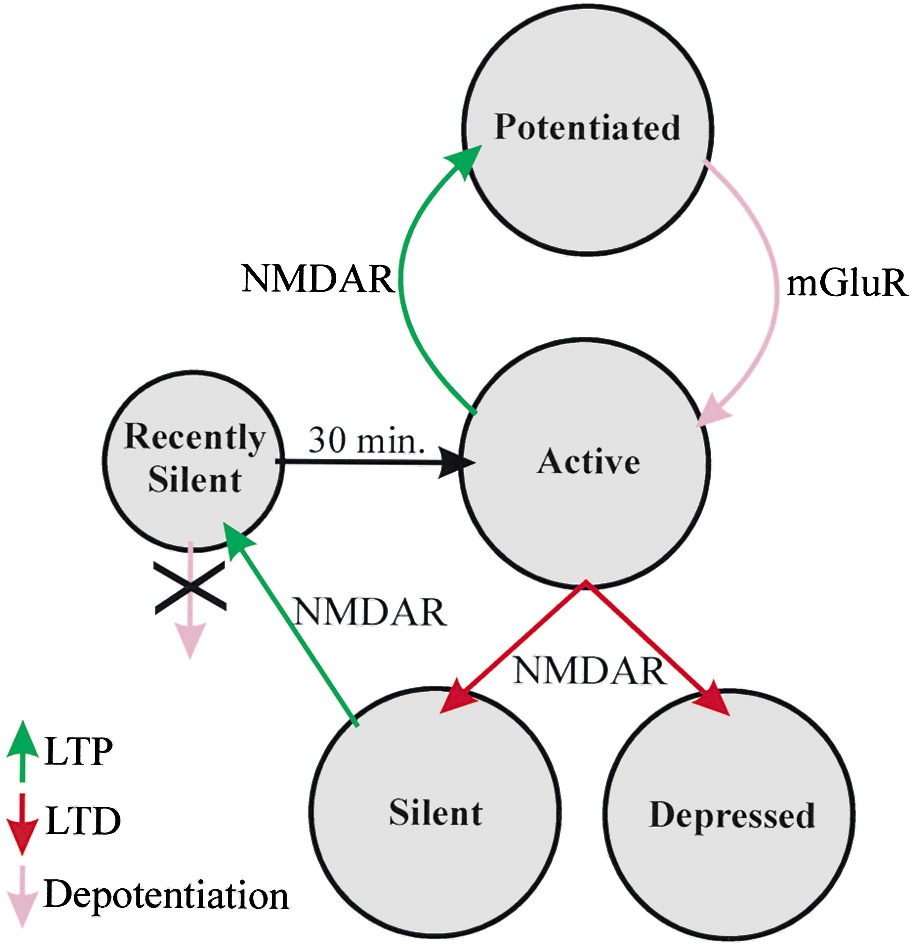
\includegraphics[height=0.8\linewidth]{MadisonMontgomery.jpg}

 \citerr{Montgomery2002765}
 }
%
\end{frame}

%-------------Slide--------------------------------------------------------

\begin{frame}{Outline}
%
 \tableofcontents%[hideallsubsections]
% \begin{itemize}
%   \item Motor learning
% \begin{itemize}
%   \vp\item Cerebellar learning of mice with enhanced plasticity
%
%   \vp\item Complex synaptic models
% \end{itemize}
%   \vp\item (Memory capacity of complex synapses)
% \end{itemize}
 %
%
\end{frame}

% ------Section------------------------------------------------------------

\section{Learning with enhanced plasticity}

%-------------Slide--------------------------------------------------------

\begin{frame}{Benefits of enhanced plasticity?}
%
 Learning requires synaptic plasticity.
 %
 \begin{center}
   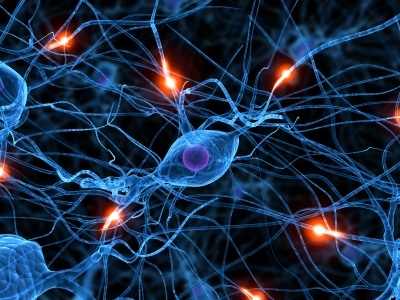
\includegraphics[width=0.4\linewidth]{NeuronsActive.jpg}
 \end{center}
 %
 Can we enhance learning by enhancing plasticity?

 \vp
 %
 \begin{center}
   \alignmid{
\includegraphics[width=0.4\linewidth]{Limitless1noblkborders.png}}
 \end{center}
 %
%
\end{frame}


%-------------Slide--------------------------------------------------------

\begin{frame}{Enhanced plasticity \texorpdfstring{\emph{can}}{can} enhance learning}
%
% \parbox[t]{0.3\linewidth}{
%   Overexpress NR2B  \\[0.5cm]
%   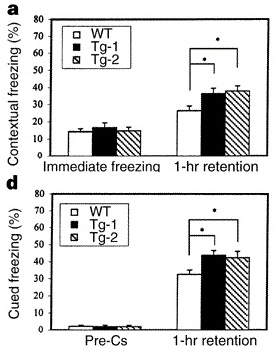
\includegraphics[width=0.97\linewidth]{enh-Tang.jpg} \\
%   Fear conditioning  \\
%   \citerr{Tang1999enhancedLearning}
% }
% \hspace{0.03\linewidth}
% \parbox[t]{0.3\linewidth}{
%   Inhibit CN \\[0.5cm]
%   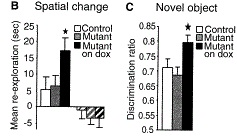
\includegraphics[width=0.97\linewidth]{enh-Malleret.jpg} \\
%   Novel object recognition \\
%   \citerr{Malleret2001enhancedLearning} \\
% }
% \hspace{0.03\linewidth}
% \parbox[t]{0.3\linewidth}{
%   Knockout Hdac2 \\[0.5cm]
%   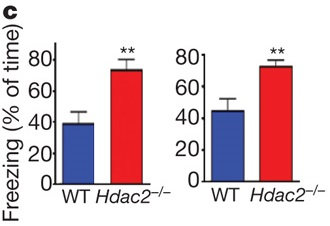
\includegraphics[width=0.97\linewidth]{enh-Guan.jpg} \\
%   Fear conditioning \\
%   \citerr{Guan2009enhancedLearning} \\
% }
 \begin{tabular}{p{0.3\linewidth}@{\hspace{0.03\linewidth}}p{0.3\linewidth}@{\hspace{0.03\linewidth}}p{0.3\linewidth}}
   % after \\: \hline or \cline{col1-col2} \cline{col3-col4} ...
   Overexpress NR2B & Inhibit CN & Knockout Hdac2 \\[0.5cm]
   \aligntop{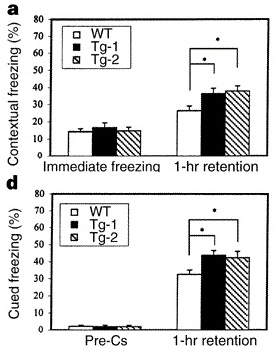
\includegraphics[width=0.7\linewidth]{enh-Tang.jpg}} &
   \aligntop{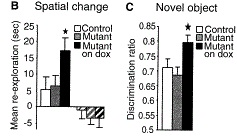
\includegraphics[width=0.97\linewidth]{enh-Malleret.jpg}} &
   \aligntop{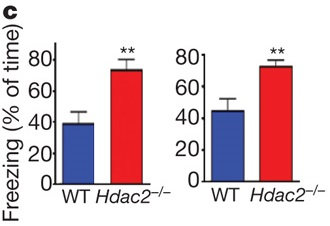
\includegraphics[width=0.97\linewidth]{enh-Guan.jpg}} \\
   Fear conditioning & Novel object recog. & Fear conditioning \\
   \citerr{Tang1999enhancedLearning} & \citerr{Malleret2001enhancedLearning} & \citerr{Guan2009enhancedLearning} \\
 \end{tabular}
%
\end{frame}

%-------------Slide--------------------------------------------------------

\begin{frame}{Enhanced plasticity can \texorpdfstring{\emph{impair}}{impair} learning}
%
 \begin{tabular}{p{0.22\linewidth}@{\hspace{0.03\linewidth}}p{0.22\linewidth}@{\hspace{0.03\linewidth}}p{0.22\linewidth}@{\hspace{0.03\linewidth}}p{0.22\linewidth}}
   % after \\: \hline or \cline{col1-col2} \cline{col3-col4} ...
   Mutate PSD-95 & Knockout PTP$\delta$ & Delete Tmod2 & Knockout FMR1 \\[0.5cm]
   \aligntop{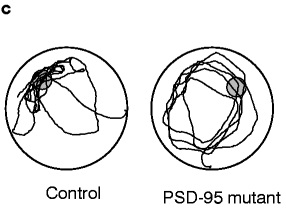
\includegraphics[width=0.7\linewidth]{imp-Migaud.jpg}} &
   \aligntop{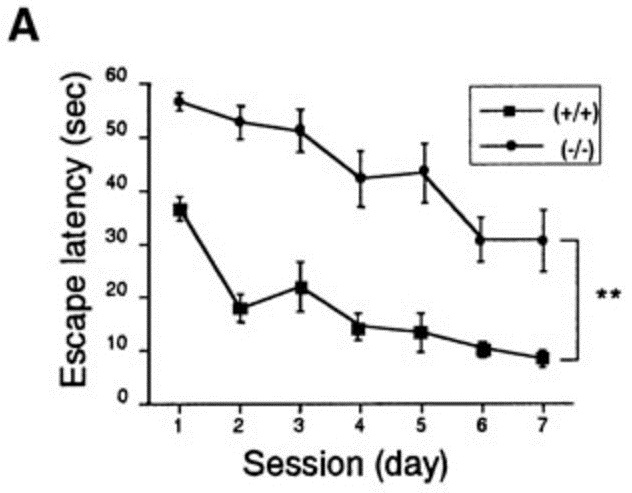
\includegraphics[width=0.97\linewidth]{imp-Uetani.jpg}} &
   \aligntop{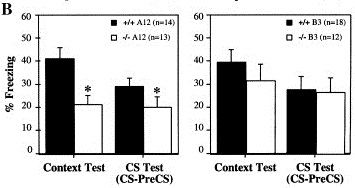
\includegraphics[width=0.97\linewidth]{imp-Cox.jpg}} &
   \aligntop{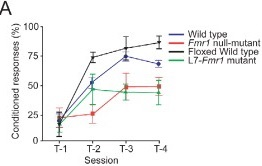
\includegraphics[width=0.97\linewidth]{imp-Koekkoek.jpg}} \\
   Water maze & Water maze & Fear cond. & Eyeblink \\
   \citerrr{Migaud1998impairedLearning} & \citerrr{Uetani2000impairedLearning} & \citerrr{Cox2003impairedLearning} & \citerrr{Koekkoek2005impairedConditioning}
 \end{tabular}

 \vp\hfill also: \citerrr{Hayashi2004impairedConsolidation,Rutten2008impairedLearning}
%
\end{frame}

%-------------Slide--------------------------------------------------------

\begin{frame}{Overview}
%
 \parbox[c]{0.8\linewidth}{%
 Sometimes enhanced plasticity \lto\ enhanced learning.\\
 Sometimes enhanced plasticity \lto\ impaired learning.

 \vp Why? How? When?}
     \hfill{\alignmid{
\includegraphics[width=0.1\linewidth]{pinky_by_lonewolf16.jpg}}} {\alignmid{
\includegraphics[width=0.07\linewidth]{the_brain_by_lonewolf16.jpg}}}

 \onslide<2->\vp Mice with enhanced cerebellar plasticity can show \alert{both} impaired and enhanced learning.
 \note[item]{Depends on circumstance. Rich pattern of behaviour}

 \vp Simple synapses \alert{cannot} explain behaviour.
 \alert{Complex synapses} are required.\\
 \lto\ predictions for synaptic physiology.
 \note[item]{Develop understanding of when and why learning is enhanced/impaired}
%
\end{frame}

%-------------Section--------------------------------------------------------

\subsection{Effects of enhanced plasticity on VOR learning}
%\subsection{VOR learning and the cerebellum}

%-------------Slide--------------------------------------------------------

\begin{frame}{Vestibulo-Occular Reflex}
%
 \parbox[t]{0.35\linewidth}{\aligntop{
\includegraphics[width=0.99\linewidth]{VOR.svg}}}
 \parbox[t]{0.64\linewidth}{%
 Eye movements compensate for head movements $\implies$ stabilise image on retina.

 \vp Requires control of $\text{VOR gain} = \frac{\text{eye velocity}}{\text{head velocity}}$.

 \vp Needs to be adjusted as eye muscles age, \etc
 }

%
\end{frame}


%-------------Slide--------------------------------------------------------

\begin{frame}{Vestibulo-Occular Reflex training}
%
\note[item]{Explain what VOR gain is}
 \parbox[t]{0.2\linewidth}{%
   \aligntop{
\includegraphics[width=0.99\linewidth]{VORinc.svg}}
     \note[item]{trick brain into thinking VOR gain needs adjusting my moving visual stimulus}
     \note[item]{anti-phase \lto\ increase gain}

   \vp\aligntop{
\includegraphics[width=0.99\linewidth]{VORdec.svg}}
     \note[item]{in phase \lto\ decrease gain}
   }
 \hspace{0.15\linewidth}
 \parbox[t]{0.59\linewidth}{%
   \aligntop{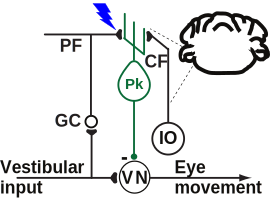
\includegraphics[width=0.99\linewidth]{VORcircuit.svg}}

%   \vp PF-Pk: \parbox[t]{0.5\linewidth}{PF+CF \lto LTD, \\
%              PF+\cancel{CF} \lto LTP.}

   \vp \begin{tabular}{ll}
   VOR increase: & LTD in PF-Pk synapses.\\
   VOR decrease: & different mechanism,\\
    & also reverses LTD in PF-Pk.
   \end{tabular}
 }
% \parbox[t]{0.59\linewidth}{%
% \raggedleft
%   \aligntop{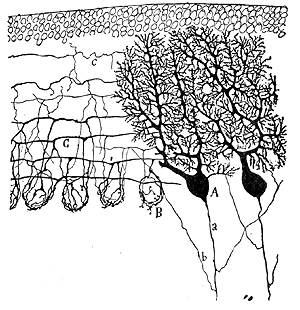
\includegraphics[width=0.5\linewidth]{pk.png}}\\
%   \rref{Cajal}
%
%   \vp \begin{tabular}{ll}
%   VOR increase: & LTD in PF-Pk synapses.\\
%   \end{tabular}
%
%   \vp  \aligntop{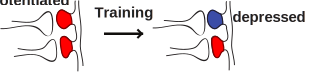
\includegraphics[width=0.8\linewidth]{ltd.svg}}
%
% }
   \note[item]{Gain change involves cerebellum}
   \note[item]{If we enhanced plasticity here: expect enhanced learning}
%   \note[item]{Marr-Albus-Ito: Pf-Pk synapses}
%   \note[item]{Lisberger-Miles: Vestibular input-VN synapses}
%   \note[item]{Different mechs for different freq, head angle, gain up/down.}
%   \note[item]{Different Pk cells have different tunings.}
%   \note[item]{Gain up in case of interest: LTD in Pf-Pk in flocculus}
%   \note[item]{Gain down: uses different mech for behaviour, but does reverse LTD in Pf-Pk in flocculus}
%   \note[item]{PF-Pk:PF+CF \lto\ LTD, PF+\cancel{CF} \lto\ LTP.}

 \citerr{Marr1969cerebellum,Albus1971cerebellum,ito1972cerebellum}
% \citerr{duLac1995review,Boyden2004review}
%
\end{frame}

%%-------------Section--------------------------------------------------------
%
%\subsection{The effects of enhanced plasticity and saturation}

%-------------Slide--------------------------------------------------------

\begin{frame}{Enhanced plasticity impairs learning}
%
 \alert{Expectation:} enhanced LTD \lto\ enhanced learning.

 \begin{center}
 \begin{tabular}{lr}
%   Baseline & \hspace{0.1\linewidth} &
%   Gain increase \\[0.5cm]
%   \alignmid{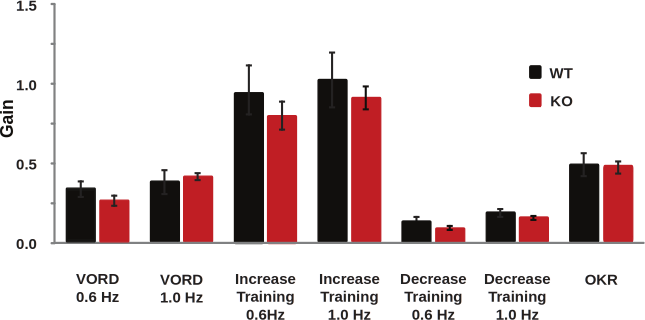
\includegraphics[width=0.4\linewidth]{baseline.svg}} &&
   \alignmid{
\includegraphics[width=0.2\linewidth]{VORinc.svg}}&
   \alignmid{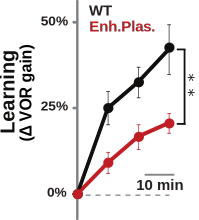
\includegraphics[width=0.3\linewidth]{gain_inc.svg}}\\
   &\alert{Experiment:} enhanced plasticity \lto\ impaired learning.
 \end{tabular}
 \end{center}
% \note[item]{No difference in baseline occulomotor performance}
 \note[item]{Impairment of learning}
 \note[item]{Looking at change of VOR gain during gain-up training}

\vp
 \note[item]{Major Histocompatibility Complex - involved in synaptic plasticity (Carla Shatz lab)}
 Knockout of MHC-I K$^\mathsf{b}$D$^\mathsf{b}$ molecules in PF-Pk synapses\\
  \lto\ lower threshold for LTD  \citerr{McConnell2009MHCcerebellum}


%
\end{frame}

%-------------Slide--------------------------------------------------------

\begin{frame}{Depletion hypothesis}
%
{}
 {\color{darkgrey} Learning rate} $\sim$ {\color{darkgreen}intrinsic plasticity rate} $\times$ {\color{darkblue}\# synapses available for LTD}.

 \vp
 \begin{center}

%   \parbox[t]{0.25\linewidth}{%\raggedright
%     \visible<1,2>{\aligntop{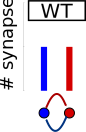
\includegraphics[height=\linewidth]{binary_bar_wt_wo_n.svg}}}
%   }
   %
   \only<1>{\aligntop{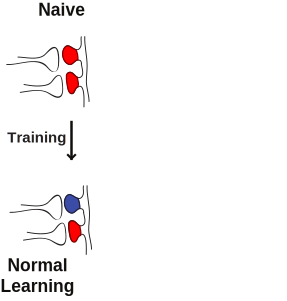
\includegraphics[width=0.5\linewidth]{sat_model_1.svg}}}%
   \only<2->{\aligntop{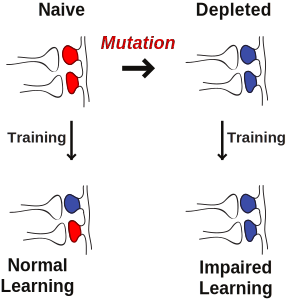
\includegraphics[width=0.5\linewidth]{sat_model_2.svg}}}%
   %
%   \hspace{0.3\linewidth}
%   %
%   \parbox[t]{0.25\linewidth}{%\raggedleft
%     \visible<2>{\aligntop{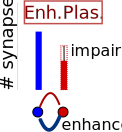
\includegraphics[height=\linewidth]{binary_bar_ko_wo_n.svg}}}
%   }

   \vp\visible<3>{\alert{Question 1:} {\color{darkblue}depletion effect} competes with {\color{darkgreen}enhanced intrinsic plasticity}.
   When is depletion effect stronger?}

% \end{tabular}
%   \vp

 \end{center}
% \note[item]{Older explanation: error model}
 \note[item]{Our model: baseline activity \lto\ saturation \lto\ less depression possible}
 \note[item]{Saturation has to compete with enhanced plasticity. Which will win?}
%
\end{frame}

%-------------Slide--------------------------------------------------------

\begin{frame}{Replenishment by reverse-training}
%
 %
 \begin{center}
   \only<1>{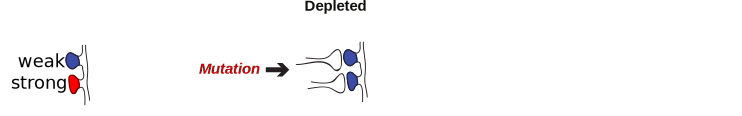
\includegraphics[width=0.7\linewidth]{desat_1.svg}}%
   \only<2>{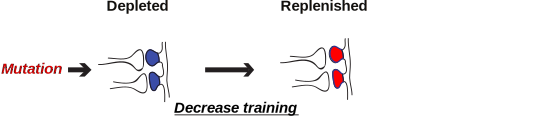
\includegraphics[width=0.7\linewidth]{desat_2.svg}}%
   \only<3->{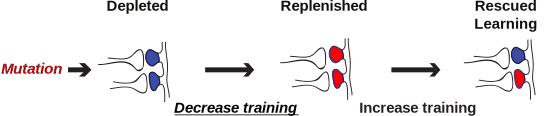
\includegraphics[width=0.7\linewidth]{desat_3.svg}}

   \vp
  \begin{overlayarea}{0.7\linewidth}{0.25\linewidth}
   \only<4>{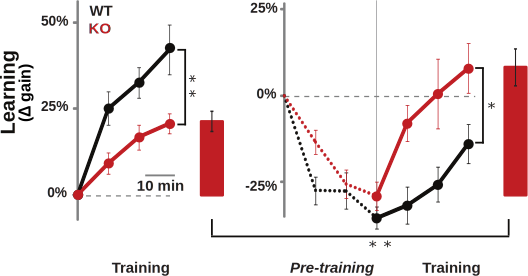
\includegraphics[width=0.9\linewidth]{gain_dec.svg}}%
%
%   \vp
   \only<5->{
   \begin{tabular}{c@{\hspace{0.2\linewidth}}c}
   \color{red!60!black}{Enh.\ Plast.} & WT \\[0.2cm]
   \aligntop{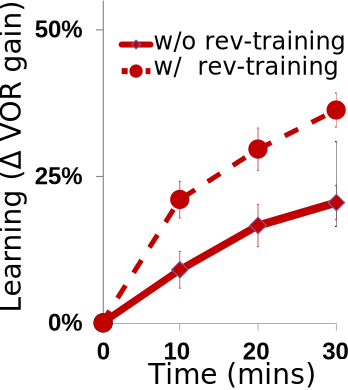
\includegraphics[width=0.35\linewidth]{data_shifted_KO.svg}}
   &
   \aligntop{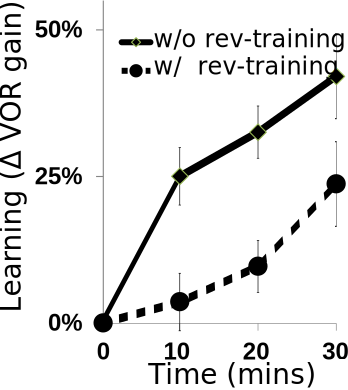
\includegraphics[width=0.35\linewidth]{data_shifted_WT.svg}}
   \end{tabular}
   }
   \end{overlayarea}
 \end{center}

 \visible<5->{\vp\alert{Question 2:} How can replenishment \emph{ever} impair learning?}
 %
 \note[item]{precede gain inc training w/ gain dec rev-training: reverses LTD}
 \note[item]{(but behaviour from elsewhere \lto\ not modelled)}
 \note[item]{Shift origin to compare}
%
\end{frame}

% -----Section-------------------------------------------------------------

\subsection{Synaptic models of VOR learning}

%%-------------Slide--------------------------------------------------------
%
%\begin{frame}{Synapses are complex}
%%
% \parbox[t]{0.45\linewidth}{%
% 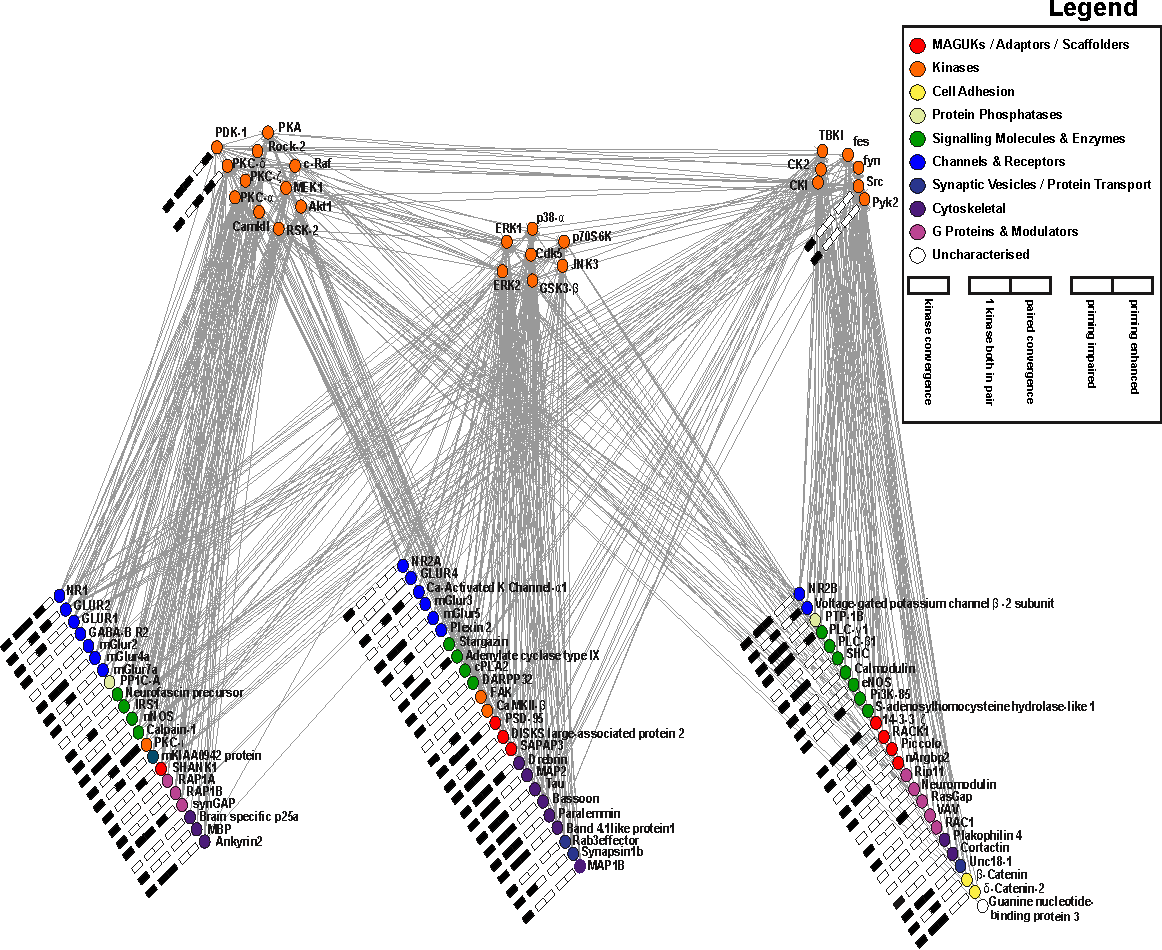
\includegraphics[height=0.8\linewidth]{2000102CobaFig4.pdf}
%
% \citerr{Coba2009phosphorylation}
% }
% \hspace{0.05\linewidth}
% \parbox[t]{0.45\linewidth}{%
% \hfill
% 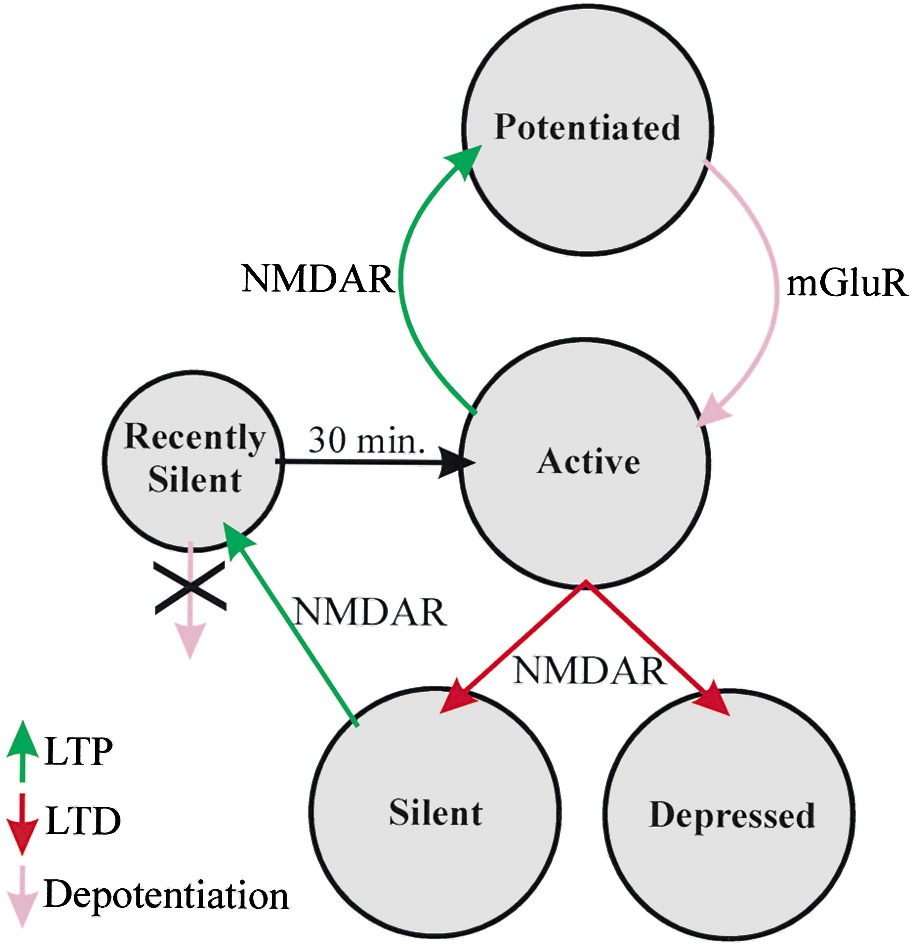
\includegraphics[height=0.8\linewidth]{MadisonMontgomery.jpg}
%
% \citerr{Montgomery2002765}
% }
%%
%\end{frame}

%-------------Slide--------------------------------------------------------

\begin{frame}{Models of complex synaptic dynamics}
%
%  There are $N$ identical synapses with $M$ internal functional states.
\visible<2->{
\parbox[c]{0.82\linewidth}{%
  \begin{itemize}
    \item Internal functional state of synapse \lto\ synaptic weight.
    \item Candidate plasticity events \lto\ transitions between states
  \end{itemize}
}\hfill
\alignmid{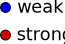
\includegraphics[width=0.13\linewidth]{state_key.svg}}
}

  %
  \vp
%  \begin{overlayarea}{0.7\linewidth}{0.3\linewidth}
%    \only<1>{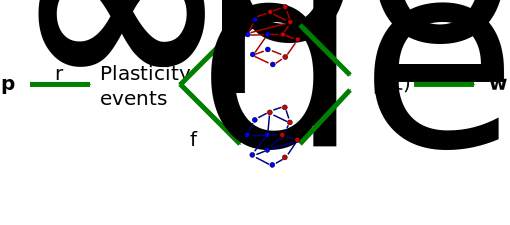
\includegraphics[width=0.99\linewidth]{synapse_model_1.svg}}%
%    \only<2>{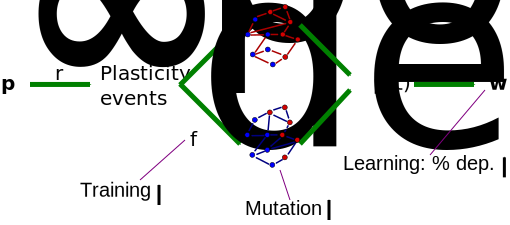
\includegraphics[width=0.99\linewidth]{synapse_model_2.svg}}
%  \end{overlayarea}
%
\begin{overlayarea}{0.95\linewidth}{0.4\textheight}
  \begin{center}
%\aligntop{\movie[width=200px,height=92px,showcontrols=true,loop]{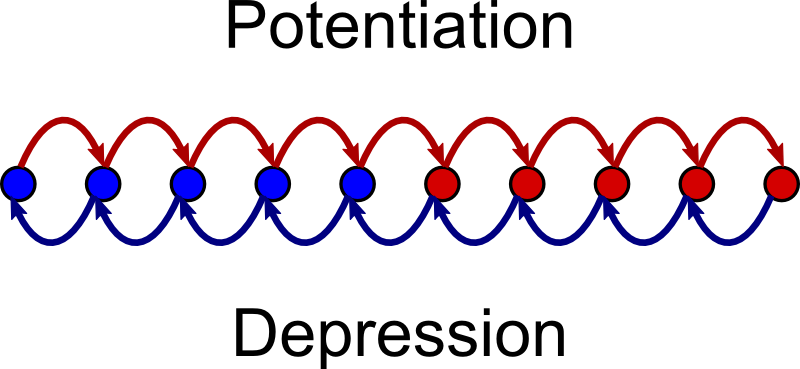
\includegraphics[width=200px,height=92px]{Vids/plast_00.png}}{plast.avi}}
    \only<1>{\aligntop{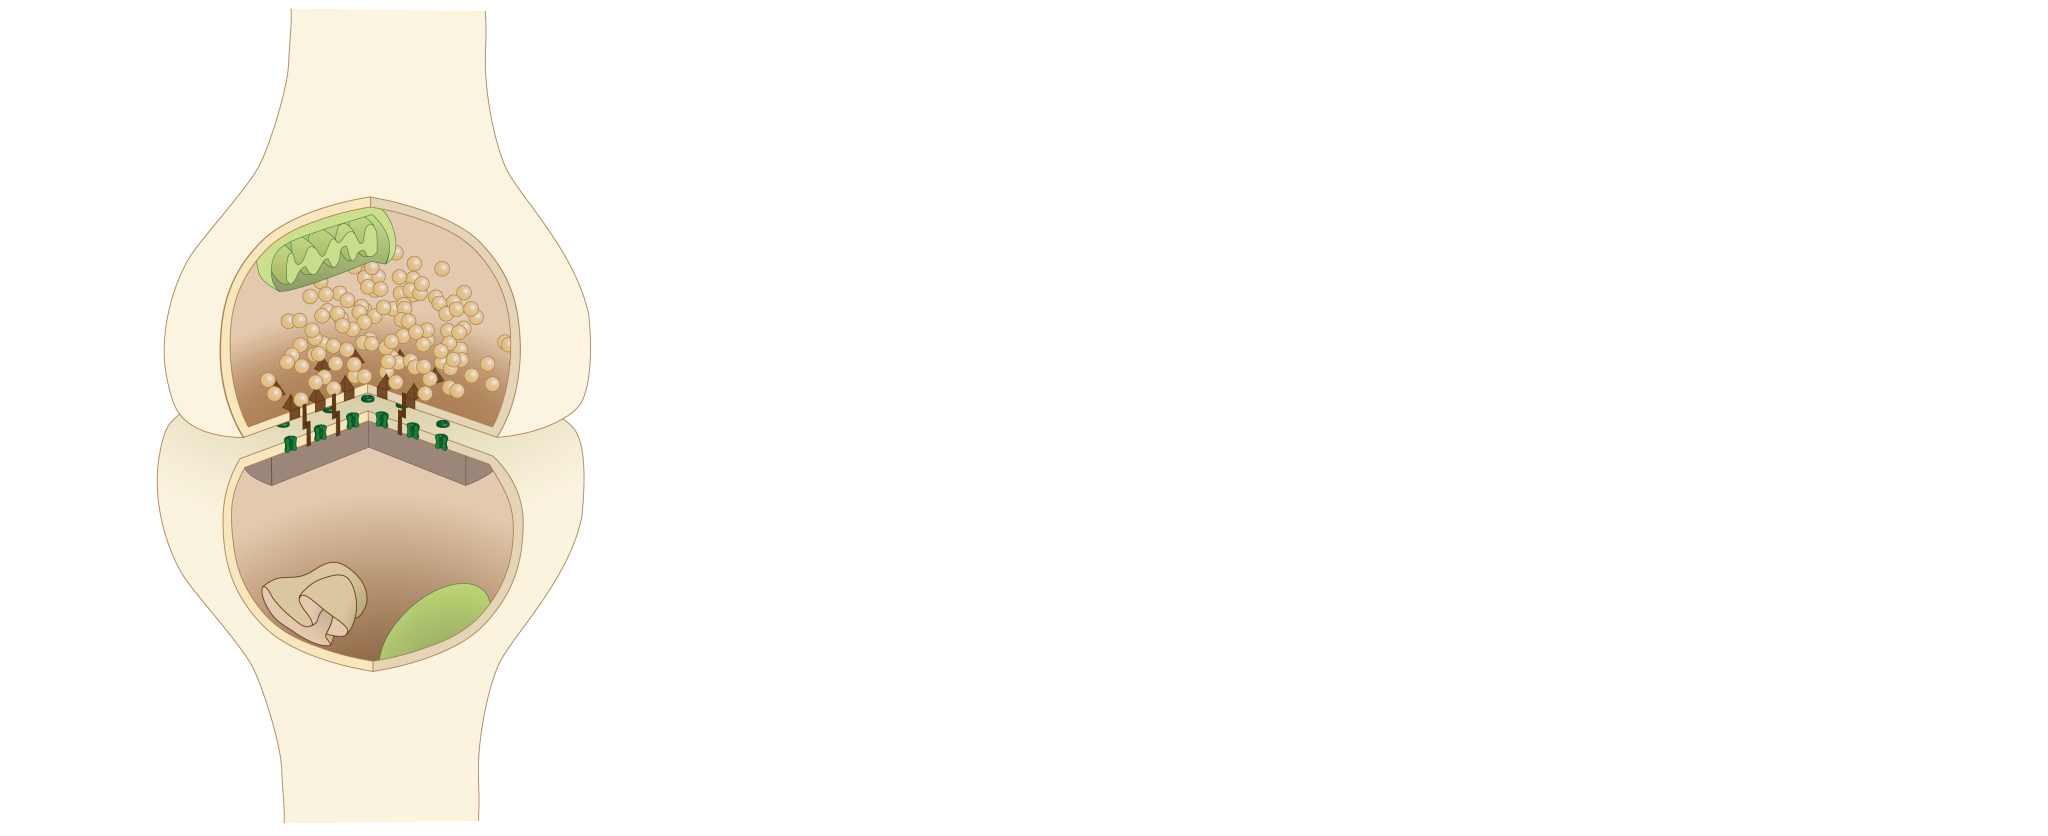
\includegraphics[width=0.7\linewidth]{serial_internal_1.svg}}}%
    \only<2>{\aligntop{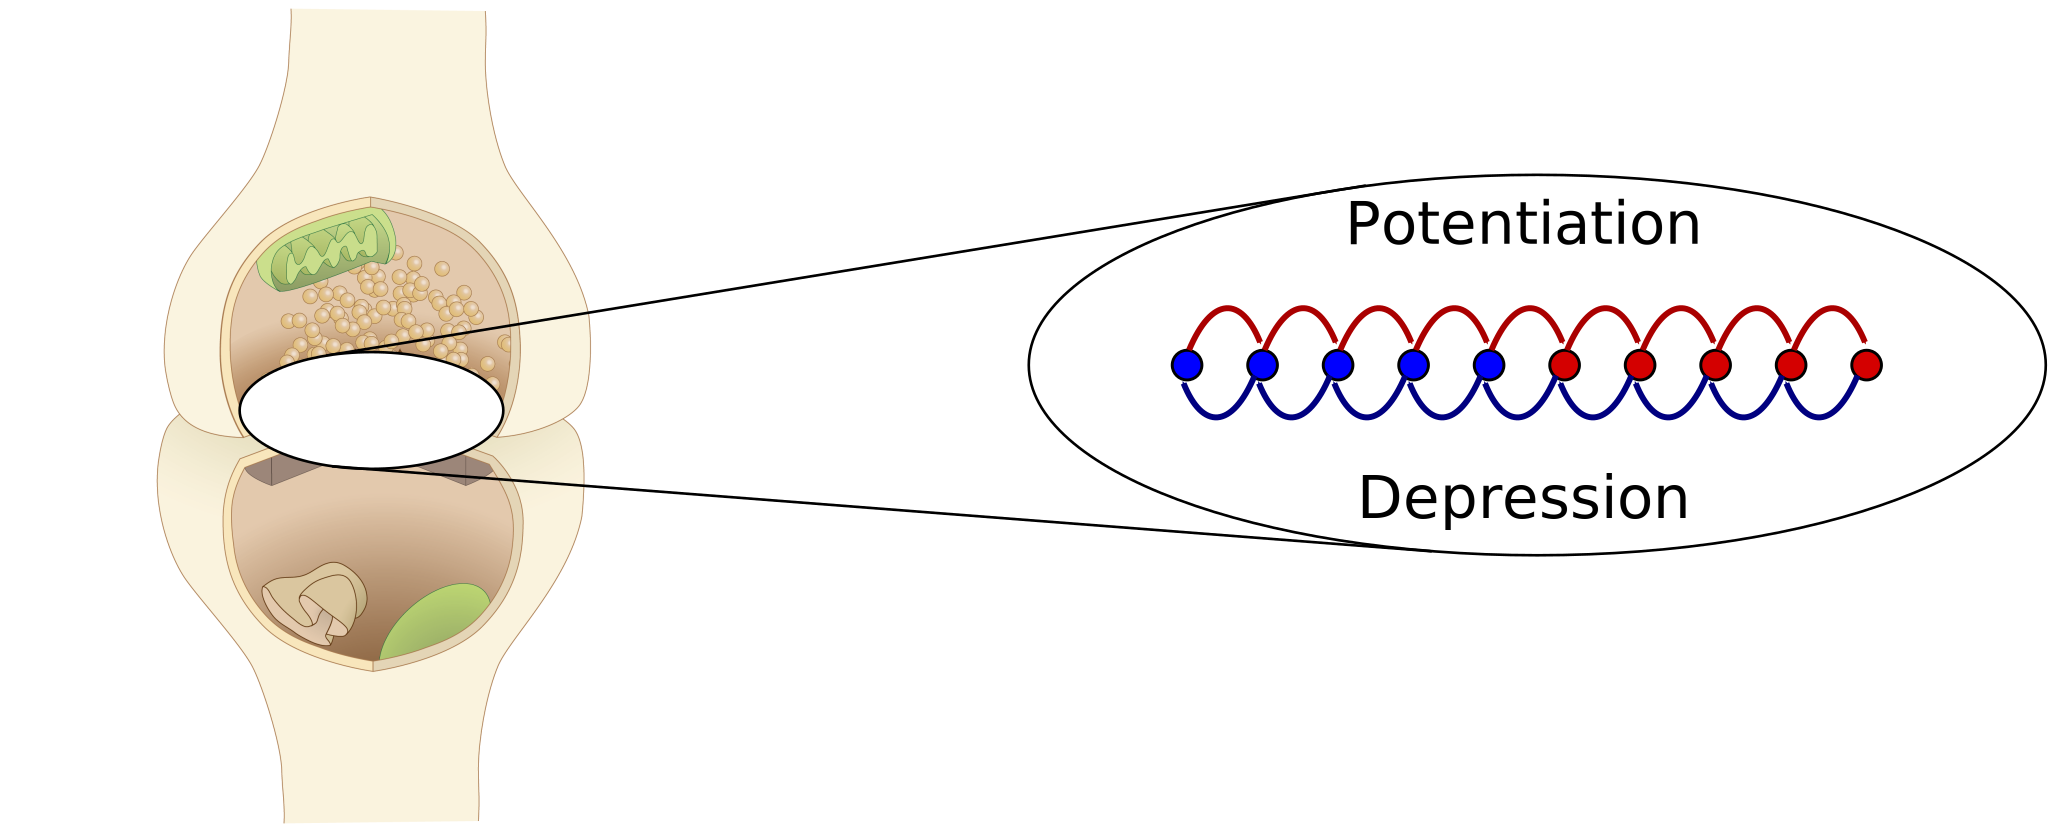
\includegraphics[width=0.7\linewidth]{serial_internal.svg}}}%
    \only<3->{\vp}
    \only<3>{\aligntop{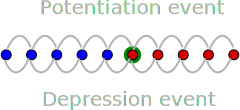
\includegraphics[width=0.5\linewidth]{Animation/serial_anim_01.svg}}}%
    \only<4>{\aligntop{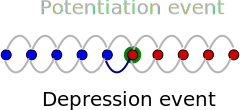
\includegraphics[width=0.5\linewidth]{Animation/serial_anim_02.svg}}}%
    \only<5>{\aligntop{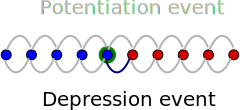
\includegraphics[width=0.5\linewidth]{Animation/serial_anim_03.svg}}}%
    \only<6>{\aligntop{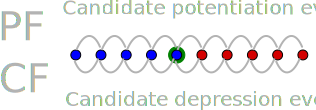
\includegraphics[width=0.5\linewidth]{Animation/serial_anim_04.svg}}}%
    \only<7>{\aligntop{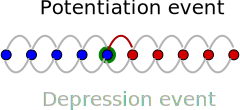
\includegraphics[width=0.5\linewidth]{Animation/serial_anim_05.svg}}}%
    \only<8>{\aligntop{\includegraphics[width=0.5\linewidth]{Animation/serial_anim_06.svg}}}%
    \only<9>{\aligntop{\includegraphics[width=0.5\linewidth]{Animation/serial_anim_07.svg}}}%
    \only<10>{\aligntop{\includegraphics[width=0.5\linewidth]{Animation/serial_anim_08.svg}}}%
    \only<11>{\aligntop{\includegraphics[width=0.5\linewidth]{Animation/serial_anim_09.svg}}}%
    \only<12>{\aligntop{\includegraphics[width=0.5\linewidth]{Animation/serial_anim_10.svg}}}%
    \only<13>{\aligntop{\includegraphics[width=0.5\linewidth]{Animation/serial_anim_11.svg}}}%
    \only<14>{\aligntop{\includegraphics[width=0.5\linewidth]{Animation/serial_anim_12.svg}}}%
    \only<15>{\aligntop{\includegraphics[width=0.5\linewidth]{Animation/serial_anim_13.svg}}}%
    \only<16>{\aligntop{\includegraphics[width=0.5\linewidth]{Animation/serial.svg}}}%
%    \only<5>{\aligntop{\includegraphics[width=0.5\linewidth]{Animation/serial_anim_06.svg}}}%
%    \only<6>{\aligntop{\includegraphics[width=0.5\linewidth]{Animation/serial_anim_07.svg}}}%
%    \only<7>{\aligntop{\includegraphics[width=0.5\linewidth]{Animation/serial_anim_08.svg}}}%
%    \only<8>{\aligntop{\includegraphics[width=0.5\linewidth]{Animation/serial_anim_09.svg}}}%
%    \only<9>{\aligntop{\includegraphics[width=0.5\linewidth]{Animation/serial_anim_10.svg}}}%
%    \only<10>{\aligntop{\includegraphics[width=0.5\linewidth]{Animation/serial_anim_11.svg}}}%
%    \only<11>{\aligntop{\includegraphics[width=0.5\linewidth]{Animation/serial_anim_12.svg}}}%
%    \only<12>{\aligntop{\includegraphics[width=0.5\linewidth]{Animation/serial_anim_13.svg}}}%
%    \only<13>{\aligntop{\includegraphics[width=0.5\linewidth]{Animation/serial.svg}}}%
    %
%    \hspace{0.05\linewidth}\parbox[t]{0.45\linewidth}{\raggedright
%    \visible<15>{
%    Mutation: transition probabilities \\ \vp
%    Training: rates of pot/dep events \\ \vp
%    Learning: synaptic weight}}
  \end{center}
\end{overlayarea}

%  \onslide<2>{\hfill
%  \parbox[t]{0.3\linewidth}{PF+\cancel{CF} \lto\ LTP, \\
%              PF+CF \lto\ LTD.}
%  \parbox[t]{0.27\linewidth}{Lower threshold\\ for LTD}
%  \parbox[t]{0.27\linewidth}{VOR gain increase}}
\vp
\begin{overlayarea}{0.95\linewidth}{0.3\textheight}
  \only<2>{States: \parbox[t]{0.85\linewidth}{NMDAR subunit composition, CaMK II autophosphorylation,\\
                                              activating PKC, p38 MAPK,...}

  \vp\footnotesize\citerr{Fusi2005cascade,Fusi2007multistate,Barrett2008discrete}\\\citerr{Smith2006savings,Lahiri2013synapse}}%

  \only<9->{Metaplasticity: \parbox[t]{0.7\linewidth}{%
     change propensity for plasticity \\
     (independent of change in synaptic weight).}}
\end{overlayarea}

  %
  \note[item]{complex synapse: not just synaptic weight. dynamical system}
  \note[item]{important for memory with bounded synapses}
  \note[item]{nodes \lto\ states}
  \note[item]{color \lto\ sttrength}
  \note[item]{arrows \lto\ plasticity}
%  \note[item]{stoch process has steady state distribution.}
%  \note[item]{Prior activity puts it in this state. row vec.}
  \note[item]{plasticity events at rate r. indep at each synapse.}
  \note[item]{fraction pot/dep}
  \note[item]{Readout: synaptic weight vec when in each state.}
    \note[item]{Mutation: lower threshold \lto\ increase transition probs}
    \note[item]{Training: Changes statistics of LTP/LTD. Only parameters we have. Don't care about $r$.}
    \note[item]{Learning: Only output we have. Don't keep track of synaptic identity.}
\end{frame}

%-------------Slide--------------------------------------------------------

\begin{frame}{Modelling VOR experiments}
%
 \visible<3->{PF-Pk LTD \lto\ VOR increase}
 %
 \begin{center}
    \only<1>{\aligntop{\includegraphics[width=0.9\linewidth]{multi-serial.svg}}}%
    \only<2>{\aligntop{\includegraphics[width=0.5\linewidth]{Animation/learn_anim_wt.svg}}}%
    \only<3>{\aligntop{\includegraphics[width=0.5\linewidth]{Animation/learn_anim_1.svg}}}%
    \only<4>{\aligntop{\includegraphics[width=0.5\linewidth]{Animation/learn_anim_21.svg}}}%
    \only<5>{\aligntop{\includegraphics[width=0.5\linewidth]{Animation/learn_anim_41.svg}}}%
    \only<6>{\aligntop{\includegraphics[width=0.5\linewidth]{Animation/learn_anim_61.svg}}}%
    \only<7>{\aligntop{\includegraphics[width=0.5\linewidth]{Animation/learn_anim_81.svg}}}%
    \only<8>{\aligntop{\includegraphics[width=0.5\linewidth]{Animation/learn_anim_101.svg}}}%
    \only<9>{\aligntop{\includegraphics[width=0.5\linewidth]{Animation/learn_anim_wt.svg}}}%
    \only<10>{\aligntop{\includegraphics[width=0.5\linewidth]{Animation/learn_anim_ko.svg}}}%

 \end{center}
 %
 \visible<3->{
 Training: \parbox[t]{0.7\linewidth}{%
 different CF activity $\implies$\\
 change frequency of pot/dep events.
 } }

 \visible<8->{
 \vp Learning: \parbox[t]{0.7\linewidth}{%
 decrease in average synaptic weight.
 } }

 \visible<9->{
 \vp Mutation: \parbox[t]{0.7\linewidth}{%
 lower threshold for LTD $\implies$\\
 increase transition probability for depression events.
 } }
%
\end{frame}

%-------------Slide--------------------------------------------------------

\begin{frame}{Questions}
%
 Depletion effect competes with enhanced intrinsic plasticity.

 \vp\alert{Question 1:}  When is the depletion effect stronger?

 \vp\vp Reverse training impairs learning in wild-type.

 \vp\alert{Question 2:} How can replenishment \emph{ever} impair learning?

 \vp\vp Enhanced plasticity \lto\ enhanced/impaired learning

 \vp\alert{Big question:} Why? When?
%
\end{frame}

% -------Section-----------------------------------------------------------

\subsection{Learning outcomes of mice and models}

%-------------Slide--------------------------------------------------------

\begin{frame}{Simple synapses cannot explain the data}
%
 \begin{center}
 \begin{tabular}{c@{\hspace{0.1\linewidth}}c}
   \only<1>{\aligntop{\includegraphics[height=0.15\linewidth]{multistate.svg}}}%
   \only<2-6>{\aligntop{\includegraphics[height=0.15\linewidth]{binary.svg}}}%
   &
   \visible<1-3,5>{\aligntop{\includegraphics[height=0.19\linewidth]{VORinc.svg}}}\\[2cm]
   \only<1>{\aligntop{\includegraphics[width=0.35\linewidth]{blank_learnS.svg}}}%
   \only<2>{\aligntop{\includegraphics[width=0.35\linewidth]{binary_learnS.svg}}}%
   \only<3>{\aligntop{\includegraphics[width=0.35\linewidth]{binary_learnS_top.svg}}}%
   \only<4>{\aligntop{\includegraphics[width=0.35\linewidth]{binary_bar_ko_wo_s.svg}}}%
   \only<5>{\aligntop{\includegraphics[width=0.35\linewidth]{binary_learnS_left.svg}}}%
   \only<6>{\aligntop{\includegraphics[width=0.35\linewidth]{binary_bar_wt_w_s.svg}}}%
   &
   \only<1-2>{\aligntop{\includegraphics[width=0.35\linewidth]{data_shifted_nl.svg}}}%
   \only<3>{\aligntop{\includegraphics[width=0.35\linewidth]{data_shifted_top_nl.svg}}}%
   \only<4>{\parbox[t]{0.35\linewidth}{\centering \vp depletion effect\\ $<$ \\ enhanced plasticity \\
   \vp $\implies$  enhanced learning}}%
   \only<5>{\aligntop{\includegraphics[width=0.35\linewidth]{data_shifted_left_nl.svg}}}%
   \only<6>{\parbox[t]{0.35\linewidth}{\centering \vp reverse training\\ $\implies$ \\ replenishment \\
    $\implies$ \\ enhanced learning}}%
 \end{tabular}
 \end{center}
 \note[item]{Binary fails -- mathematical proof for any params}
 \note[item]{Enh.Plas: faster depression wins over bias}
 \note[item]{pre: reduces/reverses bias. always helps.}
%
\end{frame}

%-------------Slide--------------------------------------------------------

\begin{frame}{Complex metaplastic synapses can explain the data}
%
 \begin{center}
 \begin{tabular}{c@{\hspace{0.1\linewidth}}c}
   \aligntop{\includegraphics[height=0.15\linewidth]{serial.svg}} &
   \visible<1,2,4>{\aligntop{\includegraphics[height=0.19\linewidth]{VORinc.svg}}}\\[2cm]
   \only<1>{\aligntop{\includegraphics[height=0.35\linewidth]{serial_fit_learnS.svg}}}%
   \only<2>{\aligntop{\includegraphics[height=0.35\linewidth]{serial_fit_learnS_top.svg}}}%
   \only<3>{\aligntop{\includegraphics[height=0.35\linewidth]{serial_bar_ko_wo_s.svg}}}%
   \only<4>{\aligntop{\includegraphics[height=0.35\linewidth]{serial_fit_learnS_left.svg}}}%
%   \only<3>{\aligntop{\includegraphics[height=0.35\linewidth]{serial_bar_ko_w_s.svg}}}%
   \only<5,6>{\aligntop{\includegraphics[height=0.35\linewidth]{serial_bar_wt_w_s.svg}}}%
   \only<7>{\parbox[t][0.343\linewidth]{0.35\linewidth}{\centering starting point:\\ labile states \\ $\downarrow$ \\
   enhanced plasticity \\ $\implies$  impaired learning}}%
   &
   \only<1>{\aligntop{\includegraphics[height=0.35\linewidth]{data_shifted_nl.svg}}}%
   \only<2>{\aligntop{\includegraphics[height=0.35\linewidth]{data_shifted_top_nl.svg}}}%
   \only<3>{\parbox[t]{0.35\linewidth}{\centering \vp amplified depletion\\ $>$ \\ enhanced plasticity \\
   \vp $\implies$  impaired learning}}%
%   \only<3>{\aligntop{\includegraphics[height=0.35\linewidth]{data_shifted_right_nl.svg}}}%
   \only<4>{\aligntop{\includegraphics[height=0.35\linewidth]{data_shifted_left_nl.svg}}}%
   \only<5>{\parbox[t]{0.35\linewidth}{\centering \vp reverse training\\ $+$ \\ ``stubborn'' metaplasticity \\
   \vp $\implies$  impaired learning}}%
   \only<6>{\aligntop{\includegraphics[height=0.35\linewidth]{serial_bar_ko_w_s.svg}}}%
   \only<7>{\parbox[t][0.343\linewidth]{0.35\linewidth}{\centering starting point:\\ stubborn states \\ $\downarrow$ \\
   enhanced plasticity \\ $\implies$  enhanced learning}}%
 \end{tabular}
 \end{center}
%  \visible<3>{\alert{Key:} ``Stubborn'' metaplasticity}\\
% \visible<1>{\citerr{Leibold2008serial,Ben-DayanRubin2007sparse}}

 \note[item]{Serial: still only two weights. Works.}
 \note[item]{Understand by looking at distributions before training}
%
\end{frame}

%-------------Slide--------------------------------------------------------

\begin{frame}{Essential features}
%
 %
 \begin{center}
   \includegraphics[width=0.4\linewidth]{serial_s.svg}
 \end{center}
 %
 \vp The success of the serial model relies on two features:
 \begin{itemize}
   \item Complexity - needed for depletion to dominate enhanced plasticity,
   \note[item]{due to exponential decay}
   \item Stubbornness - repeated potentiation impairs subsequent depression.
   \note[item]{push away from boundary where signal generated}
 \end{itemize}
 \note[item]{borne out by other models that fail/succeed}

 %\visible<2>{
 \begin{center}
 \begin{tabular}{c@{\hp\hp}c}
    Fail:&
    Succeed:\\[0.3cm]
    \aligntop{\includegraphics[width=0.3\linewidth]{pooled_s.svg}}&
    \aligntop{\includegraphics[width=0.3\linewidth]{cascade_s.svg}}\\[1.5cm]
    \aligntop{\includegraphics[width=0.3\linewidth]{multistate_s.svg}}&
    \aligntop{\includegraphics[width=0.3\linewidth]{multistate_nonuni_s.svg}}
 \end{tabular}
 \end{center}
 %\citerr{amit1994learning,Fusi2005cascade}
 %}
%
\end{frame}

%-------------Slide--------------------------------------------------------

\begin{frame}{Conclusions}
%
 \begin{itemize}
%   \item The saturation effect can overcome faster depression, if it is enhanced.
%   \alert{Requires complexity}
%   \note[item]{\eg exponential deacy, resource depletion,\ldots}
%   \item A little reverse bias can help, but too much hurts, if repeated potentiation makes depression harder.
%   \alert{Requires metaplasticity}
%   \note[item]{\eg moving away from weight boundary, or weaker transitions.}
   \item Diverse behavioural patterns:\\
   \alert{Enhanced plasticity \lto\ enhance/impair} learning (prior experience).\\
   \alert{Reverse-training \lto\ enhance/impair} learning (plasticity rates).

   \item \alert{enhanced LTD} vs.\ \alert{depletion} \lto\ learning outcome.
    \hfill{\alignmid{\includegraphics[width=0.1\linewidth]{pinky_by_lonewolf16.jpg}}} {\alignmid{\includegraphics[width=0.07\linewidth]{the_brain_by_lonewolf16.jpg}}}



   \item Predictions for synaptic physiology:\\
   \alert{Complexity:} necessary to amplify depletion.\\
   \alert{Stubbornness:} repeated potentiation impairs subsequent depression.

   \vp\item  We used behaviour to constrain the dynamics of synaptic plasticity.
\end{itemize}
%
\end{frame}


% -------Section-----------------------------------------------------------

\section{Memory over different timescales}

%-------------Slide--------------------------------------------------------

\begin{frame}{Storage capacity of synaptic memory}
%
  Hopfield, perceptron have capacity $\propto N$, (\# synapses).

\vp\parbox[t]{0.59\linewidth}{%
  Assumes unbounded analog synapses
  %Requires synapses' dynamic range also $\propto N$.

 \vp With discrete, finite synapses:\\
 $\implies$ memory capacity  $\sim\CO(\log N)$.
 \\ \citerr{amit1992constraints,amit1994learning}
 %
 }
 %
 \parbox[t]{0.4\linewidth}{
   %\begin{flushright}
    \hfill\aligntop{\includegraphics[width=0.9\linewidth]{Petersen1998.jpg}}
   %\end{flushright}
 }
 \\
    \citerr{Petersen1998allornone,OConnor2005switch}

 \vp New memories overwrite old
 $\implies$ stability-plasticity dilemma.
 %
 \note[item]{or sparse $\sim \log N / N$}
%
\end{frame}


%-------------Slide--------------------------------------------------------

\begin{frame}{Models of complex synaptic dynamics}
%
  There are $N$ identical synapses with $M$ internal functional states.
%
\parbox[c]{0.82\linewidth}{%
  \begin{itemize}
    \item Internal functional state of synapse \lto\ synaptic weight.
    \item Candidate plasticity events \lto\ transitions between states
  \end{itemize}
}\hfill
\alignmid{\includegraphics[width=0.13\linewidth]{state_key.svg}}
%

  \begin{center}
    \aligntop{\includegraphics[width=0.6\linewidth]{synapse_internal.svg}}
%    \hspace{0.07\linewidth}
%    \aligntop{\includegraphics[width=0.3\linewidth]{MadisonMontgomery.jpg}}
%    \\ \citerr{Montgomery2002765}
  \end{center}

  States: \parbox[t]{0.85\linewidth}{\#AMPAR, \#NMDAR, NMDAR subunit composition, \\
  CaMK II autophosphorylation, activating PKC, p38 MAPK,...}

  \vp \footnotesize\citerr{Fusi2005cascade,Fusi2007multistate,Barrett2008discrete}%%\\\citerr{Smith2006savings,Lahiri2013synapse}}%
  %
  \note[item]{complex synapse: not just synaptic weight. dynamical system}
  \note[item]{important for memory with bounded synapses}
  \note[item]{nodes \lto\ states}
  \note[item]{color \lto\ sttrength}
  \note[item]{arrows \lto\ plasticity}
%  \note[item]{stoch process has steady state distribution.}
%  \note[item]{Prior activity puts it in this state. row vec.}
  \note[item]{plasticity events at rate r. indep at each synapse.}
  \note[item]{fraction pot/dep}
  \note[item]{Readout: synaptic weight vec when in each state.}
  %
\end{frame}

%-------------Slide--------------------------------------------------------

\begin{frame}{Specific models of complex synaptic dynamics}
%
  \begin{center}
    \parbox[t]{0.4\linewidth}{\aligntop{\includegraphics[width=0.95\linewidth]{cascade.svg}}
                               \par\citerr{Fusi2005cascade}}
    \hspace{0.05\linewidth}
    \parbox[t]{0.4\linewidth}{\aligntop{\includegraphics[width=0.95\linewidth]{serial.svg}}
                               \par\citerr{Ben-DayanRubin2007sparse} \par\citerr{Leibold2008serial}}

    \vp
    \parbox[t]{0.4\linewidth}{\aligntop{\includegraphics[width=0.95\linewidth]{BennaFusi.svg}}
                               \par\citerr{Benna2015complex}}
    \hspace{0.05\linewidth}
    \parbox[t]{0.4\linewidth}{\aligntop{\includegraphics[width=0.95\linewidth]{integ_express.pdf}}
                               \par\citerr{Elliott2011}}
  \end{center}
%
\end{frame}

% ----Section--------------------------------------------------------------

\subsection{Quantifying memory quality}

%%-------------Slide--------------------------------------------------------
%
%
%\begin{frame}{Recognition memory}
%%
% Synapses given a sequence of patterns (pot \& dep) to store
%
% %\vp
% \begin{center}
% \only<1>{\aligntop{\includegraphics[width=0.275\linewidth]{perceptron1.svg}}}%
% \only<2>{\aligntop{\includegraphics[width=0.275\linewidth]{perceptron2.svg}}}%
%% \only<3>{\aligntop{\includegraphics[width=0.275\linewidth]{perceptron3.svg}}}%
% \only<3>{\aligntop{\includegraphics[width=0.275\linewidth]{perceptron4.svg}}}%
%% \only<5>{\aligntop{\includegraphics[width=0.275\linewidth]{perceptron5.svg}}}%
% \only<4>{\aligntop{\includegraphics[width=0.275\linewidth]{perceptron6.svg}}}%
%% \only<7>{\aligntop{\includegraphics[width=0.275\linewidth]{perceptron7.svg}}}%
% \only<5->{\aligntop{\includegraphics[width=0.275\linewidth]{perceptron8.svg}}}%
% \end{center}
%
% \visible<5->{Later: presented with a pattern.
% Has it been seen before?
%%
%
% \vp Compare $\synid \cdt \syn(t)$ to threshold.
% \citerr{Sommer1998retrieval}}
% %
% \visible<6>{%
% %
% \begin{equation*}
%     \snr(t) = \frac{ \av{\synid\cdt\syn(t)} - \av{\synid\cdt\syn(\infty)} }{ \sqrt{\var(\synid\cdt\syn(\infty))}},
%     \qquad
%     \snrb(\tau) = \intd{\tau} \frac{\e^{-t/\tau}}{\tau} \snr(t).
% \end{equation*}
%}
%%
%\end{frame}
%
%
%-------------Slide--------------------------------------------------------

\begin{frame}{Synaptic memory curves}
%
 %
 \begin{center}
   \includegraphics[width=0.5\linewidth]{MemorySequence.svg}
 \end{center}
 %
 Synapses store a sequence of memories.\\
 Recognition memory performance described by SNR.
 %
 \begin{center}
   {\includegraphics[width=0.55\linewidth]{MemoryCurve.svg}}
 \end{center}
 %
%
\end{frame}

%-------------Slide--------------------------------------------------------

\begin{frame}{General principles relating structure and function?}
%
 \vspace{-2\baselineskip}
 \begin{center}
 \parbox[t]{0.35\linewidth}{%
 \begin{center}
   Synaptic structure\\
   \includegraphics[width=0.99\linewidth]{synapse_internal.svg}
 \end{center}
 }
 \hspace{0.1\linewidth}
 \parbox[t]{0.3\linewidth}{%
 \begin{center}
   Synaptic function\\
   \includegraphics[width=0.99\linewidth]{MemoryCurve.svg}
 \end{center}
 }
 \end{center}
 \begin{itemize}
   \item What are the fundamental limits of memory?
   \vp\item Which models achieve these limits?
   \vp\item What are the theoretical principles behind the optimal models?
 \end{itemize}
%
\end{frame}


%-------------Slide--------------------------------------------------------

\begin{frame}{Parameters for synaptic dynamics}
%
%  There are $N$ identical synapses with $M$ internal functional states.
%  %
%  \begin{center}
%    \includegraphics[width=0.7\linewidth]{model.svg}
%  \end{center}
%  %
%  \note[item]{stoch process has steady state.}
%  \note[item]{Prior activity puts it in this state. row vec.}
%  \note[item]{plasticity events at rate r}
%  \note[item]{fraction pot/dep}
%  \note[item]{probs changed by Markov matrices, prob $i\to j$}
%  \note[item]{Readout: synaptic weight vec when in each state.}
%  \vp
% At $t=0$, the memory is created by $\M\potdep$ with probability $f\potdep$.
% \note[item]{for this one, we keep track of pot/dep, look for inc/dec of $\w$}
%
  %
  \begin{equation*}
  \begin{aligned}
     \alert{f\potdep} &= \text{fraction of events that are pot/dep,} \\
    \text{pot. event: } \alert{M\pot_{ij}} &= \text{transition prob. } i \to j, \quad  
    &{\scriptstyle
    \W\pot =  f\pot \prn{\M\pot - I},} \\
    \text{dep. event: } \alert{M\dep_{ij}} &= \text{transition prob. } i \to j, \quad   
    &{\scriptstyle
    \W\dep =  f\dep \prn{\M\dep - I}.} \\
  \end{aligned}
  \end{equation*}
%
 Constraints:
 %
 \begin{equation*}
   f\potdep, \M\potdep_{ij} \in [0,1], \qquad
   f\pot + f\dep = \sum_j \M\potdep_{ij} = 1.
 \end{equation*}
 %
 \note[item]{difficult to to apply}
 \note[item]{Memory at $t=0$, keep track of pot/dep}
 \note[item]{subsequent: average over pot/dep}
 \note[item]{$\frg$ is forgetting matrix, $\I=$identity, don't keep track of pot/dep}
%
%
 Memory curve given by
 %
 \begin{equation*}
 \begin{aligned}
%    \frg &= f\pot\M\pot+f\dep\M\dep-\I, \qquad
%    \eq \frg =0, \\
   \snrb(\tau)
        &= \sqrt{N}\, \eq \prn{\W\pot-\W\dep} \brk{\I - r\tau\prn{\W\pot + \W\dep}}\inv \w. \\
        &= \sqrt{N}\sum_a \frac{\initial_a }{1+r \tau / \tau_a}. \\
  %
 \end{aligned}
 %
 \end{equation*}
 %
 \note[item]{prefactors don't do anything, ignore}
 \note[item]{prior state, encoding, forgetting, readout}

%
\end{frame}

% ----------------------------------------------------------------

\subsection{Frontiers of memory}

%-------------Slide--------------------------------------------------------

\begin{frame}{Upper bounds on measures of memory}
%
\parbox[t]{0.6\linewidth}{
 Initial SNR:
 %
 \begin{equation*}
   \initial = \snr(0) = \sum_a \initial_a \leq \sqrt{N}.
 \end{equation*}
 %
 %
 \begin{center}
   \includegraphics[height=0.1\linewidth]{binary_det.svg}
 \end{center}
 %
 }
 \parbox[t]{0.39\linewidth}{
    \aligntop{\includegraphics[width=0.96\linewidth]{snr_props.svg}}
 } \par
 Area under curve:
 %
 \begin{equation*}
   \area = \int_0^\infty \!\snr(t)\, \dt = \sum_a \initial_a \tau_a \leq \sqrt{N}(M-1)/r.
 \end{equation*}
 %
 %
 \begin{center}
   \includegraphics[height=0.1\linewidth]{multistate_sticky.svg}
 \end{center}
 %
 \citerr{Lahiri2013synapse}
%
\end{frame}

%-------------Slide--------------------------------------------------------

\begin{frame}{Proven envelope: memory frontier}
%
 \visible<1->{Upper bound on memory curve at \emph{any} timescale.}

 %\vp
 \begin{center}
% \parbox[c]{0.67\linewidth}{
   %\only<1>{\aligntop{\includegraphics[width=0.95\linewidth]{RunAveProvenNum2.svg}}}%
   \only<1>{\aligntop{\includegraphics[width=0.67\linewidth]{RunAveProvenNum1.svg}}}%
   \only<2>{\aligntop{\includegraphics[width=0.67\linewidth]{RunAveProvenNum.svg}}}%
   \note[item]{Best we've found, by numerical opt and hand chosen models.}
% \note[item]{Models on next slide}
% }
 \end{center}
% \hspace{0.01\linewidth}
 %
% \visible<3>{
% \parbox[c]{0.3\linewidth}{
%   Serial topology:
%   %
%   \begin{center}
%  %   \includegraphics[width=6cm]{multistate_shorten.svg}
%     \includegraphics[width=0.99\linewidth]{multistate.svg}
%   \end{center}
%   %
% }}
 \note[item]{Gap $\sim\CO(\sqrt{N})$.}
 \note[item]{Area bound active at early times $\implies$ need more constraints.}
%
\end{frame}


%-------------Slide--------------------------------------------------------

\begin{frame}{Models that maximize memory for one timescale}
%
 %
 \parbox[c]{0.67\linewidth}{
 \begin{center}
   \only<1>{\aligntop{\includegraphics[width=0.9\linewidth]{RunAveModels1.svg}}}%
   \only<2>{\aligntop{\includegraphics[width=0.9\linewidth]{RunAveModels2.svg}}}%
   \only<3>{\aligntop{\includegraphics[width=0.9\linewidth]{RunAveModels3.svg}}}%
 \end{center}
 }
%
 \parbox[c]{0.3\linewidth}{
   %
   \begin{center}
     \visible<1>{\includegraphics[width=0.99\linewidth]{multistate_uni4.svg}}
     \visible<2>{\includegraphics[width=0.99\linewidth]{multistate_uni.svg}}
     \visible<3>{\includegraphics[width=0.99\linewidth]{multistate_sticky.svg}}
   \end{center}
   %
 }

%
\end{frame}


%%-------------Slide--------------------------------------------------------
%
%\begin{frame}{Models that maximise memory for one timescale}
%%
% %
% \begin{center}
%   \only<1>{\aligntop{\includegraphics[width=0.9\linewidth]{Animation/Lenv27.svg}}}%
%   %\only<2>{\aligntop{\includegraphics[width=0.9\linewidth]{Animation/Lenv30.svg}}}%
%   \only<2>{\aligntop{\includegraphics[width=0.9\linewidth]{Animation/Lenv34.svg}}}%
%   %\only<2>{\aligntop{\includegraphics[width=0.9\linewidth]{Animation/Lenv42.svg}}}%
%   \only<3>{\aligntop{\includegraphics[width=0.9\linewidth]{Animation/Lenv47.svg}}}%
%   %\only<6>{\aligntop{\includegraphics[width=0.9\linewidth]{Animation/Lenv51.svg}}}%
%   %
%   \only<4>{\aligntop{\includegraphics[width=0.9\linewidth]{Animation/Lenv27.svg}}}%
%   %\only<8>{\aligntop{\includegraphics[width=0.9\linewidth]{Animation/Lenv24.svg}}}%
%   %\only<9>{\aligntop{\includegraphics[width=0.9\linewidth]{Animation/Lenv21.svg}}}%
%   \only<5>{\aligntop{\includegraphics[width=0.9\linewidth]{Animation/Lenv20.svg}}}%
%   %\only<11>{\aligntop{\includegraphics[width=0.9\linewidth]{Animation/Lenv19.svg}}}%
%   %\only<12>{\aligntop{\includegraphics[width=0.9\linewidth]{Animation/Lenv17.svg}}}%
%   \only<6>{\aligntop{\includegraphics[width=0.9\linewidth]{Animation/Lenv16.svg}}}%
%   %\only<14>{\aligntop{\includegraphics[width=0.9\linewidth]{Animation/Lenv14.svg}}}%
%   %\only<15>{\aligntop{\includegraphics[width=0.9\linewidth]{Animation/Lenv12.svg}}}%
%   \only<7>{\aligntop{\includegraphics[width=0.9\linewidth]{Animation/Lenv06.svg}}}%
%   %\only<17>{\aligntop{\includegraphics[width=0.9\linewidth]{Animation/Lenv01.svg}}}%
% \end{center}
%%
%%
%\end{frame}
%
%
%-------------Slide--------------------------------------------------------
%
%\begin{frame}{Heuristic envelope}
%%
% %
% \begin{center}
%   \includegraphics[width=0.88\linewidth]{LenvAnalytic.svg}
% \end{center}
%%
%%
%\end{frame}

% ----------------------------------------------------------------

\subsection{Implications of memory limits}

%-------------Slide--------------------------------------------------------

\begin{frame}{Synaptic diversity and timescales of memory}
%
 \parbox[t][][t]{0.47\linewidth}{
 Different synapses have different molecular structures.
 \begin{center}
   \aligntop{\includegraphics[width=0.8\linewidth]{Emes2012.jpeg}}
 \end{center}
 \citerr{Emes2012synapserev}
 }
 %
 \hspace{0.03\linewidth}
 %
 \visible<2->{%
 \parbox[t][][t]{0.47\linewidth}{
 Memories stored in different places for different timescales

 \citerr{Squire1995amnesia}

 \citerr{McClelland1995consolidation}
 \begin{center}
   \aligntop{\includegraphics[width=0.9\linewidth]{sleepconsolidation.png}}
 \end{center}
 \citerr{Born2012sleep}

 Also: Cerebellar cortex \lto\ nuclei.

 \citerr{Attwell2002consolidation}

 \citerr{Cooke2004consolidation}
 }}
 %
%
\end{frame}

%-------------Slide--------------------------------------------------------

\begin{frame}{Synaptic structure and function: general principles}
%
 Real synapses limited by molecular building blocks. \\
 Evolution had larger set of priorities.

 \vp What can we conclude?

 \begin{center}
 \begin{tabular}{ccccc}
   % after \\: \hline or \cline{col1-col2} \cline{col3-col4} ...
   Short timescale & $\longrightarrow$ & Moderate timescale & $\longrightarrow$ & Long timescale \\[0.5cm]
   \alignmid{\includegraphics[height=0.064\linewidth]{multistate_uni4.svg}} & $\longrightarrow$ & \alignmid{\includegraphics[height=0.064\linewidth]{multistate_uni.svg}} & $\longrightarrow$ & \alignmid{\includegraphics[height=0.064\linewidth]{multistate_sticky.svg}} \\[0.5cm]
   \visible<2->{short topology} & \visible<2->{$\longrightarrow$} & \visible<2->{long topology} &  &  \\[0.5cm]
    & & \visible<3->{deterministic synapse} & \visible<3->{$\longrightarrow$} & \visible<3->{stochastic synapse} \\
 \end{tabular}
 \end{center}
%
\end{frame}

% ----------------------------------------------------------------

\section{Designing experiments}

%-------------Slide--------------------------------------------------------

\begin{frame}{Experimental tests?}
%
 Traditional experiments:

 \begin{center}
     \aligntop{\includegraphics[width=0.7\linewidth]{barrage.svg}}%
 \end{center}

 \vp\visible<2>{To fit a model: long sequence of small plasticity events.

 Observe the changes in synaptic efficacy.}

 \begin{center}
     \visible<2>{\aligntop{\includegraphics[width=0.7\linewidth]{gentle.svg}}}%
 \end{center}

% \visible<7->{\textbf{EM algorithms:}
%
%   Sequence of hidden states $\ra$ estimate transition probabilities \\
%   Transition probabilities $\ra$ estimate sequence of hidden states
%
%   \citerr{Baum1970baumwelch,rabiner1993speechrec,Dempster2007EM}
%
% \vp \textbf{Spectral algorithms:}
%
% Compute $P(w_1), P(w_1,w_2), P(w_1,w_2,w_3),\ldots$  \hp
% \parbox[t]{0.3\linewidth}{
%   from data, \\
%   from model.
% }
%
% \citerr{Hsu2008hmmspec}
% }
%
\end{frame}

%-------------Slide--------------------------------------------------------

\begin{frame}{Simulated experiment}
%
 %
 \begin{center}
%   \only<1>{\aligntop{\includegraphics[width=0.97\linewidth]{Animation/FitVid00.svg}}}%
%   \only<2>{\aligntop{\includegraphics[width=0.97\linewidth]{Animation/FitVid104.svg}}}%
%   \only<3>{\aligntop{\includegraphics[width=0.97\linewidth]{Animation/FitVid208.svg}}}%
%   \only<4>{\aligntop{\includegraphics[width=0.97\linewidth]{Animation/FitVid312.svg}}}%
%   \only<5>{\aligntop{\includegraphics[width=0.97\linewidth]{Animation/FitVid416.svg}}}%
%   \only<6>{\aligntop{\includegraphics[width=0.97\linewidth]{Animation/FitVid520.svg}}}%
%   \only<7>{\aligntop{\includegraphics[width=0.97\linewidth]{Animation/FitVid624.svg}}}%
%   \only<8>{\aligntop{\includegraphics[width=0.97\linewidth]{Animation/FitVid728.svg}}}%
%   \only<9>{\aligntop{\includegraphics[width=0.97\linewidth]{Animation/FitVid832.svg}}}%
%   \only<10>{\aligntop{\includegraphics[width=0.97\linewidth]{Animation/FitVid939.svg}}}%
   \only<1>{\aligntop{\includegraphics[width=0.97\linewidth]{Animation/FitVid00.svg}}}%
   \only<2>{\aligntop{\includegraphics[width=0.97\linewidth]{Animation/FitVid104.svg}}}%
%   \only<3>{\aligntop{\includegraphics[width=0.97\linewidth]{Animation/FitVid208.svg}}}%
   \only<3>{\aligntop{\includegraphics[width=0.97\linewidth]{Animation/FitVid312.svg}}}%
%   \only<5>{\aligntop{\includegraphics[width=0.97\linewidth]{Animation/FitVid416.svg}}}%
   \only<4>{\aligntop{\includegraphics[width=0.97\linewidth]{Animation/FitVid520.svg}}}%
%   \only<7>{\aligntop{\includegraphics[width=0.97\linewidth]{Animation/FitVid624.svg}}}%
%   \only<5>{\aligntop{\includegraphics[width=0.97\linewidth]{Animation/FitVid728.svg}}}%
%   \only<9>{\aligntop{\includegraphics[width=0.97\linewidth]{Animation/FitVid832.svg}}}%
   \only<5>{\aligntop{\includegraphics[width=0.97\linewidth]{Animation/FitVid939.svg}}}%
 \end{center}
 %
 \textbf{EM algorithms:}

   Sequence of hidden states $\ra$ estimate transition probabilities \\
   Transition probabilities $\ra$ estimate sequence of hidden states

   \citerr{Baum1970baumwelch,rabiner1993speechrec,Dempster2007EM}

 \vp \textbf{Spectral algorithms:}

 Compute $P(w_1), P(w_1,w_2), P(w_1,w_2,w_3),\ldots$  \hp
 \parbox[t]{0.3\linewidth}{
   from data, \\
   from model.
 }

 \citerr{Hsu2008hmmspec}

%
\end{frame}


%-------------Slide--------------------------------------------------------

\begin{frame}{Experimental problems}
%
 \begin{itemize}
   \item Need single synapses.
   \item Need long sequences of plasticity events.
   \item Need to control types of candidate plasticity events.
   \item Need to measure synaptic efficacies.
 \end{itemize}

 \vp When we patch the postsynaptic neuron \lto\ Ca washout.
%
\end{frame}

%-------------Slide--------------------------------------------------------

\begin{frame}{Summary}
%
  \begin{itemize}
    \item We have formulated a general theory of learning and memory with complex synapses.
%    \item We can impose an order on the internal states of a synapse through the theory of first passage times.
%    \item The area under the memory curve of any model $<$ linear chain with same equilibrium distribution.
    \vp\item We find a memory envelope: a single curve that cannot be exceeded by the memory curve of \emph{any} synaptic model.
%    \vp\item Synaptic complexity ($M$ internal states) raises the memory envelope linearly in $M$ for times $> \CO(M^2)$.
    \vp\item We understood which types of synaptic structure are useful for storing memories for different timescales.
%    \item Gap between envelope and what we can achieve at early times?
%    \item Trade-off between SNR at different times?
%    \item For times $< \CO(M^2)$: conjecture that the model that reaches the envelope uses deterministic transitions $\to$ diffusive forgetting.
    \vp\item We studied more than a single model. We studied \emph{all possible models}, to extract general principles relating synaptic structure to function
  \end{itemize}

%
\end{frame}


%================================================================================
%-------------Slide--------------------------------------------------------

\begin{frame}{Acknowledgements}
%
\begin{tabular}{lll}
  \textbf{Surya Ganguli} & Niru Maheswaranathan & \textbf{Jennifer Raymond} \\
  Jascha Sohl-Dickstein  & Ben Poole            & \alert{Barbara Nguyen-Vu} \\
  Friedemann Zenke       & Kiah Hardcastle      & \alert{Grace Zhao}        \\
  Sam Ocko               & Lane McIntosh        & Aparna Suvrathan          \\
  Stephane Deny          & Alex Williams        & Rhea Kimpo                \\
  Jonathan Kadmon        & Christopher Stock    \\
  Madhu Advani           & Sarah Harvey         & \textbf{Carla Shatz}      \\
  Peiran Gao             & Aran Nayebi          & Hanmi Lee                 \\
  \\
  David Sussillo         & Stefano Fusi         & Marcus Benna    \\
\end{tabular}

 \vp\textbf{Funding}: Swartz Foundation, Stanford Bio-X Genentech fellowship.

% \vp\textbf{Travel grant}: Gatsby Charitable Foundation,
%                           Qualcomm Incorporated,
%                           Brain Corporation,
%                           Evolved Machines.
%    \stoppagecounthere
%
\end{frame}

%-------------Bonus--------------------------------------------------------
\appendix
%-------------Bonus--------------------------------------------------------

%-------------Slide--------------------------------------------------------

\begin{frame}{Model of circuit}
%
 %
 \begin{center}
   \includegraphics[width=0.9\linewidth]{VORmodel.svg}
 \end{center}
 %
 \note[item]{Contralateral baseline shift compensates for Our baseline shift}
 \note[item]{Gain increase due to LTD at lightning}
 \note[item]{Gain decease due to plasticity elsewhere, but also reverses LTD at lightning.}
 \note[item]{Nonlinearity here won't affect our questions, as long as it doesn't change}
 \note[item]{Nonlinearity before compensation could change things}
%
\end{frame}

%-------------Slide--------------------------------------------------------

\begin{frame}{Baseline}
%
    \includegraphics[width=0.6\linewidth]{baseline.svg}

%
\end{frame}

%-------------Slide--------------------------------------------------------

\begin{frame}{Evidence: level of depression}
%
 \aligntop{\includegraphics[width=0.45\linewidth]{pSer880.svg}}
 \hp
 \parbox[t]{0.45\linewidth}{%
 Basal level of GluR2 phosphorylation at serine 880 in AMPA receptor.

 \vp Biochemical signature of PF-Pk LTD.

 \vp Shows that \# depressed synapses in flocculus is larger in KO than WT.
 \note[item]{Predicted by saturation hypothesis}
 }
%
\end{frame}

%-------------Slide--------------------------------------------------------

\begin{frame}{Evidence: saturation by CF stimulation}
%
 Use Channelrhodopsin to stimulate CF \parbox[t]{0.45\linewidth}{%
 \lto increase LTD in PF-Pk synapses \\
 \lto simulate saturation in WT.
 }
 \note[item]{should result in similar behaviour to KO}

 \vp\begin{center}
   \alignmid{\includegraphics[width=0.3\linewidth]{CFstim.svg}}
   \hspace{0.05\linewidth}
   \alignmid{\includegraphics[width=0.3\linewidth]{CFstim_results.svg}}
   \hspace{0.05\linewidth}
   \alignmid{\includegraphics[width=0.2\linewidth]{CFstim_pSer880.svg}}
 \end{center}
%
\end{frame}

%-------------Slide--------------------------------------------------------

\begin{frame}{Other models that fail}
%
 \begin{tabular}{ll}
   % & for next tab, \\ for new line...
    \aligntop{\includegraphics[width=0.4\linewidth]{multistate.svg}}\hspace{1.5cm} &
    \aligntop{\includegraphics[width=0.28\linewidth]{multistate_learnS.eps}}
    \note[item]{MS: linear weights, unlike serial.}
    \note[item]{like bunch of binary synapses in series.}
    \note[item]{solid curves: fails early on , but catches up quickly}
    \note[item]{black curves: fails badly}
    \note[item]{No real enhancement of saturation, no metaplasticity.}
    \note[item]{All transitions contribute: pushing to end has little effect.}
    \\[2cm]
    \aligntop{\includegraphics[width=0.4\linewidth]{pooled.svg}} &
    \aligntop{\includegraphics[width=0.28\linewidth]{pooled_scarce_learnS.eps}}
    \note[item]{Pooled: resource depleted by pot/dep. replenished by reverse.}
    \note[item]{solid curves succeed: enhanced saturation}
    \note[item]{black curves fail: opposite metaplasticity, pot makes dep easier}
 \end{tabular}

 \citerr{amit1994learning}
%
\end{frame}

%-------------Slide--------------------------------------------------------

\begin{frame}{Other models that work}
%
 \begin{tabular}{ll}
   % & for next tab, \\ for new line...
    \aligntop{\includegraphics[width=0.4\linewidth]{multistate_nonuni.svg}}\hspace{1.5cm} &
    \aligntop{\includegraphics[width=0.28\linewidth]{nonuni_fit_learnS.eps}} \\[2cm]
    \aligntop{\includegraphics[width=0.4\linewidth]{cascade.svg}} &
    \aligntop{\includegraphics[width=0.28\linewidth]{cascade_fit_learnS.eps}}
 \end{tabular}
 \note[item]{Both models, trans probs decay exponentially from centre.}
 \note[item]{Nonuni: linear weights. Cascade: binary weights.}
 \note[item]{Enhanced saturation and metaplasticity}
 \note[item]{Pushing to end makes pot and dep harder}
 \note[item]{Note: hidden states not necessary}

 \citerr{Fusi2005cascade}
%
\end{frame}

%-------------Slide--------------------------------------------------------

\begin{frame}{Mathematical explanation}
%
 %
 \begin{center}
   \includegraphics[width=0.4\linewidth]{serial_label.svg}
 \end{center}
 %
 \vp Serial synapse: $\eq_i \sim \CN \prn{\frac{q\pot}{q\dep}}^i$.

 \vp Learning rate $\sim \eq_{M/2}\prn{\frac{q\dep}{q\pot}} = \CN \prn{\frac{q\pot}{q\dep}}^{\frac{M}{2}-1}$.
 \note[item]{Detailed balance. Exponential decay.}

 \vp For $M>2$: larger $q\dep \implies$ slower learning.
 \note[item]{for large enough $M,q\pot$, overcome $\CN$}

 \vp For $M=2$: larger $q\dep \implies$ larger $\CN \implies$ faster learning.
 \note[item]{Other factor in $\eq$ smaller $\implies \CN$ larger.}
%
\end{frame}

%-------------Slide--------------------------------------------------------

\begin{frame}{Quantifying memory quality}
%
% Have we seen pattern before?
 Test if $\synid \cdot \syn(t) \gtrless \theta$?

% $\synid \cdot \syn(\infty) \sim$  null distribution
% $\implies$ ROC curve:

 \vp
 \parbox[t]{0.4\linewidth}{%
 \aligntop{\includegraphics[width=0.9\linewidth]{roc.svg}}
 }
 %
 \parbox[t]{0.55\linewidth}{%
 \vspace{-\baselineskip}
 %
 \begin{equation*}
   \begin{aligned}
%   \operatorname{TPR} &= \Phi \prn{ \frac{ \snr(t) +\Phi\inv(\operatorname{FPR}) }{ \operatorname{NNR}(t) } }, \\[0.5cm]
   %\quad\text{where } \quad
     %\Phi(x) &= \int_{-\infty}^x \frac{ \e^{-\frac{z^2}{2}} }{ \sqrt{2\pi} }\, \dr z, \\
     \snr(t) &= \frac{ \av{\synid\cdt\syn(t)} - \av{\synid\cdt\syn(\infty)} }{ \sqrt{\var(\synid\cdt\syn(\infty))}}, 
     \\[\baselineskip]
     \snrb(\tau) &= \intd{\tau} \frac{\e^{-t/\tau}}{\tau} \snr(t).
     \\[\baselineskip]
     \color{darkgrey} \operatorname{NNR}(t) &= \color{darkgrey} \sqrt{\frac{ \var(\synid\cdt\syn(t)) }{ \var(\synid\cdt\syn(\infty)) }}.
   \end{aligned}
 \end{equation*}
 }
 Also: KL divergence, Chernoff distance, \ldots
%
\end{frame}

%-------------Slide--------------------------------------------------------

\begin{frame}{Initial SNR as flux}
%
 Initial SNR is closely related to flux between strong \& weak states
 %
 \note[item]{flux = eq prob $\times$ trans prob}
 %
 \begin{equation*}
   \SNR(0) \leq \frac{4\sqrt{N}}{r}\,\F_{-+}.
 \end{equation*}
 %
 \note[item]{usually saturated: pot never dec, dep never inc}
 Max when {\parbox[t]{8cm}{potentiation guarantees $\w\to+1$,\\
 depression guarantees $\w\to-1$.}}
 %
 \begin{center}
   \includegraphics[height=3cm]{max_init_pot.svg}
   \hp \hp
   \includegraphics[height=3cm]{max_init_dep.svg}
 \end{center}
 %
 \note[item]{transitions out of one node sum to 1}
 \note[item]{equivalent to two-state model: doesn't matter which strong/weak state, same prob of going to other set.}
%
\end{frame}

%-------------Slide--------------------------------------------------------

\begin{frame}{Two-state model}
%
 Two-state model equivalent to previous slide:
  \begin{center}
  Transitions:
   \parbox{2cm}{\includegraphics[height=2cm]{binary_det.svg}}
   $\implies\snr(t)=\sqrt{N}\,(4 f\pot f\dep)\,\e^{-rt}.$
  \end{center}
  \note[item]{decays very quickly}

 \vp Maximal initial SNR:\note[item]{$f\pot=\half$}
 %
 \begin{equation*}
   \snr(0) \leq \sqrt{N}.
 \end{equation*}
 %
 \note[item]{Initial SNR not a good thing to optimise.}
%
\end{frame}

%-------------Slide--------------------------------------------------------

\begin{frame}{Area under memory curve}
%
  %
  \begin{equation*}
    \area = \intd[_0^\infty]{t} \snr(t),
    \qquad
    \snrb(\tau) \ra \frac{\area}{\tau}
    \quad \text{as} \quad \tau \ra \infty.
  \end{equation*}
%


  \vp\parbox{5cm}{
  Area bounds memory lifetime:\\
  %
  \begin{equation*}
  \begin{aligned}
    \SNR(\text{lifetime})&=1
    \\
    \implies
    \quad
    \text{lifetime} &< \area.
  \end{aligned}
  \end{equation*}
  %
  }
  \parbox{6.5cm}{
    \includegraphics[width=6cm]{lifetime.eps}
  }
  %
  \note[item]{lifetime = area under green < area under blue}
  \note[item]{capacity $\sim r$ lifetime, \#new memories before we forget original.}

  %
  \vp This area has an upper bound:
  %
  \begin{equation*}
    \area \leq \sqrt{N}(M-1)/r.
  \end{equation*}
  %
  \note[item]{reminder: $N=$\#synapses, $M=$\#states}
  Saturated by a model with linear chain topology.
  \note[item]{proof next slide}
%
\end{frame}

%-------------Slide--------------------------------------------------------

\begin{frame}[label=fr_areaproof]{Proof of area bound}
%
 For any model, we can construct perturbations that
 \parbox[c]{5cm}{
  \begin{itemize}
    \item preserve equilibrium distribution,
    \item increase area.
  \end{itemize}
  \hyperlink{fr_tech}{\beamerbutton{details}}
  %
  \note[item]{relies on order \& technical condition}
 }
 \parbox[c]{5cm}{
  %
  \begin{center}
    \includegraphics[width=4cm]{shortcut.svg}
  \end{center}
  %
 }\\
 \eg decrease ``shortcut'' transitions, increase bypassed ``direct'' ones.\\
 Endpoint: linear chain

 \vp The area of this model is
 %
 \begin{equation*}
   A = \frac{2\sqrt{N}}{r}\sum_k \eq_k \abs{k-\av{k}}.
 \end{equation*}
 %
 \note[item]{max given $\eq$}
 \note[item]{now max \wrt $\eq$}
 Max: equilibrium probability distribution concentrated at both ends.
 \note[item]{keep c.o.m.\ in middle}
 \\
 \citerr{Barrett2008discrete}
 \note[item]{similar result, slightly different conditions: linear weights, mutual info}
%
\end{frame}

%-------------Slide--------------------------------------------------------

\begin{frame}{Saturating model}
%
 Make end states ``sticky''
 %
 \begin{center}
   \includegraphics[width=8cm]{multistate_sticky.svg}
 \end{center}
 %
 Has long decay time, but terrible initial SNR.
 %
 \note[item]{Difficult to get out of end state.}
 \note[item]{Area not a good thing to optimise}
 %
 \begin{equation*}
   \lim_{\varepsilon\to0}A=\sqrt{N}(M-1)/r.
 \end{equation*}
 %
%
\end{frame}

%-------------Slide--------------------------------------------------------

\begin{frame}[label=fr_tech]{Technical detail: ordering states}
%
 Let $\fpt_{ij}=$ mean first passage time from state $i$ to state $j$.
 Then:
 %
 \begin{equation*}
   \eta = \sum_j \fpt_{ij} \eq_j,
 \end{equation*}
 %
 is independent of the initial state $i$
 (Kemeney's constant).\\ \citerr{kemeny1960finite}

 \vp We define:
 %
 \begin{equation*}
   \eta^+_i = \sum_{j\in\text{strong}} \fpt_{ij} \eq_j,
   \qquad
   \eta^-_i = \sum_{j\in\text{weak}} \fpt_{ij} \eq_j.
 \end{equation*}
 %
 \note[item]{Measure ``distance'' to the strong/weak states.}
 They can be used to arrange the states in an order (increasing $\eta^-$ or decreasing $\eta^+$).
 \hyperlink{fr_areaproof}{\beamerbutton{back}}
 \note[item]{sum to constant, $\implies$ two orders same}
%
\end{frame}

%-------------Slide--------------------------------------------------------

\begin{frame}{Technical detail: upper/lower triangular}
%
 With states in order:
 %
 \begin{center}
   \includegraphics[width=2cm]{triangular_right.svg}
   \hp \hp \hp
   \includegraphics[width=2cm]{triangular_left.svg}
 \end{center}
 %
 \note[item]{pot \& dep with same initial \& final state}
 Endpoint: potentiation goes right, depression goes left.
 \note[item]{pot/dep matrices are upper/lower triangular.}
 \note[item]{one other pert. too technical, even for bonus slide!}

 \hyperlink{fr_areaproof}{\beamerbutton{back}}
%
\end{frame}

%-------------Slide--------------------------------------------------------

\begin{frame}{Intuition for using topology}
%
 %
 \begin{center}
   \includegraphics[width=0.5\linewidth]{serial_sym_label.svg}
 \end{center}
%
%
\begin{equation*}
  \begin{aligned}
    \initial &\propto q,
    &\quad
    \max_a \tau_a &\propto \frac{1}{q}, \\
    \initial &\propto \frac{1}{M},
    &
    \max_a \tau_a &\propto M^2, \\
  \end{aligned}
  %
  \quad\implies\quad
  %
  \begin{aligned}
    &\text{Stochasticity:} & \initial &\propto \frac{1}{\tau\lmax}, \\
    &\text{Topology:}      & \initial &\propto \frac{1}{\sqrt{\tau\lmax}}.
  \end{aligned}
\end{equation*}
%

%
\end{frame}

%================================================================================
%-------------Bibliography-------------------------------------------------
\begin{frame}[allowframebreaks]{References}
%

 {\small
 \bibliographystyle{unsrt_slides}
 \bibliography{maths,neuro,markov}
 }
%
\end{frame}


%-----End----------------------------------------------------------------

\end{document}
